\documentclass[uplatex, dvipdfmx]{jsarticle}

% --- 数学・統計 ---
\usepackage{amsmath, amssymb, amsthm}
\usepackage{bm}
\usepackage{mathtools}
\usepackage{enumitem}
\mathtoolsset{showonlyrefs=true}
\usepackage{mathrsfs}


% --- 図表 ---
\usepackage{tikz}
\usetikzlibrary{arrows.meta, positioning, calc}
\usepackage{graphicx}
\usepackage{float}
\usepackage{booktabs}
\usepackage[margin=25mm]{geometry}

% --- リンク ---
\usepackage{hyperref}
\usepackage{pxjahyper}

% --- tcolorbox (枠を作るパッケージ) ---
\usepackage{tcolorbox}
\tcbuselibrary{theorems, skins, breakable}

\tcbset{
  simple_style/.style={
    enhanced,
    breakable,
    frame hidden,
    colback=white,
    boxrule=0pt,
    boxsep=0pt,
    left=0pt,
    right=0pt,
    top=0pt,
    bottom=0pt,
    before skip=15pt,
    after skip=15pt,
    notitle,
  }
}

% --- カウンターを共通化する設定 ---

% 1. まずベースとなる「定義」を作る（これが親になります）
\newtcolorbox[auto counter, number within=section]{defn}[2][]{
  simple_style,
  before upper={\noindent\textbf{定義~\thetcbcounter：#2}\par\smallskip},
  #1
}

% 2. 「定理」は「定義」のカウンターを引き継ぐ
\newtcolorbox[use counter from=defn]{thm}[2][]{
  simple_style,
  before upper={\noindent\textbf{定理~\thetcbcounter：#2}\par\smallskip},
  #1
}

% 3. 「命題」も引き継ぐ
\newtcolorbox[use counter from=defn]{prop}[2][]{
  simple_style,
  before upper={\noindent\textbf{命題~\thetcbcounter：#2}\par\smallskip},
  #1
}

\newtcolorbox[use counter from=defn]{cor}[2][]{
  simple_style,
  before upper={\noindent\textbf{係~\thetcbcounter：#2}\par\smallskip},
  #1
}

% 4. 「例」も引き継ぐ（左線あり）
\newtcolorbox[use counter from=defn]{exm}[2][]{
  simple_style,
  left=8pt,
  borderline west={0.5mm}{0pt}{black!30},
  before upper={\noindent\textbf{例~\thetcbcounter：#2}\par\smallskip},
  #1
}

\begin{document}

\section{なぜPearl流が必要か}
\subsection{因果とは何か}
「相関は因果を意味しない」これは多くの統計学の教科書に書かれている初等的な注意である.しかし，実際に単なる相関と因果の違いを説明するのは困難である.
これに対して，Rubinは次の平均処置効果(Average Treatment Effect: ATE)を因果効果として定義した.
\[
  ATE = E[Y^{(1)}-Y^{(0)}].
\]
ここで，$Y^{(1)}, Y^{(0)}$はポテンシャルアウトカムと呼ばれる変数である.
よく知られているように，Rubinの因果推論では，ポテンシャルアウトカムは同時に観測されず片方は必ず欠測するという欠測問題として因果推論の問題をとらえる.
この定義は式で書くと非常に明快であるが，因果と相関の違いは何かという根本的な問いに答えられていないようにも感じる.

\subsection{回帰係数は因果を意味するか}
我々が統計学や因果推論に期待することの一つは意思決定への寄与である.
つまり，原因となる変数が1単位変われば結果はいくら変わるのかという点である.
これは，直感的に単なる相関ではなく因果関係を要求することは想像に難くない.

何千回と擦られた例であるが，アイスクリームの消費量と溺死者数は因果関係でなく相関関係である.
つまり，行政の介入によりアイスクリームの流通を規制したとしても溺死者数を下げる結果には至らない.

\begin{figure}[htbp]
  \centering
  \includegraphics[width=0.8\columnwidth]{picture_1.png}
  \caption{アイスクリームの消費量と月別の溺死者数}
  \label{fig:picture_1}
\end{figure}

ところで，「原因となる変数が1変われば結果がいくら変わるのか」という文言は目的変数を説明変数で回帰したときの回帰係数の解釈として根付いている.
図\ref{fig:picture_1}を見れば，回帰係数は$0.04$であるから「アイスクリームの消費量を100円減らせば溺死者数が4人減る」という解釈ができる.

これは相関の意味では正しいといえるが，因果の意味では正しいとは言えない.換言すれば，観察の結果としての予測としては正しいが，原因に対する介入によって得られる結果の予測ではない.

線形回帰モデルの回帰係数に期待することが因果関係である場合，観察から得られた説明変数を全投入あるいはAICやBICによって変数選択することは得策とは言えない.

次のようなデータ生成を考えよう.
\begin{align}
  &\varepsilon_X, \varepsilon_Y, \varepsilon_1, \dots, \varepsilon_6 \overset{\text{i.i.d.}}{\sim} N(0, 1) \\
  X  &= 0.6Z_1 + 0.6Z_5 + \varepsilon_X \\
  Y  &= X + 0.6Z_2 + 0.6Z_3 + 0.6Z_6 + \varepsilon_Y \\
  Z_1 &= 0.6Z_2 + \varepsilon_1 \\
  Z_2 &= \varepsilon_2 \\
  Z_3 &= 0.5X + \varepsilon_3 \\
  Z_4 &= 0.7X + 0.7Y + \varepsilon_4 \\
  Z_5 &= \varepsilon_5 \\
  Z_6 &= \varepsilon_6 
\end{align}
ここで，変数そのものが$\varepsilon$として与えられた変数を\textbf{外生変数}という.
式では見にくいため，左辺を結果，右辺を原因として原因から結果へ矢線を引いて変数の関係を視覚的に表したグラフがG(図\ref{fig:dag_1})である.
\begin{figure}[htbp]
  \centering
  \begin{tikzpicture}[
    node_var/.style={circle, draw=none, minimum size=1cm, font=\large\bfseries},
    edge_path/.style={->, >=stealth, thick},
    node distance=2.0cm and 2.0cm
  ] 
    \node[node_var] (X) {$X$};
    \node[node_var, right=4.0cm of X] (Y) {$Y$};

    \node[node_var, above right=1.0cm of X] (Z1) {$Z_1$};
    \node[node_var, right=1.0cm of Z1] (Z2) {$Z_2$};

    \node[node_var, below right=of X, yshift=1.0cm] (Z3) {$Z_3$};
    \node[node_var, below right=of X] (Z4) {$Z_4$};

    \node[node_var, left=1.0cm of X] (Z5) {$Z_5$};
    \node[node_var, right=1.0cm of Y] (Z6) {$Z_6$};

    \node[node_var, above left=of X, yshift=-1.0cm] (G) {$G$};

    \draw[edge_path] (X) to (Y);
    \draw[edge_path] (Z2) to (Z1);
    \draw[edge_path] (Z1) to (X);
    \draw[edge_path] (Z2) to (Y); 

    \draw[edge_path] (X) to (Z3);
    \draw[edge_path] (Z3) to (Y);

    \draw[edge_path] (X) to (Z4); 
    \draw[edge_path] (Y) to (Z4);

    \draw[edge_path] (Z5) to (X);
    \draw[edge_path] (Z6) to (Y);
  \end{tikzpicture}
  \caption{データの生成過程}
  \label{fig:dag_1}
\end{figure}

図\ref{fig:dag_1}を見れば，どの矢線に沿って移動したとしても一周していないことが分かる.
これは，因果関係には原因と結果があり，一方向にしか進まないというある種哲学的な要請である.
このように頂点間の関係に向きがあり，どの矢線に沿って移動しても一周しないグラフを\textbf{非巡回有向グラフ}(Directed Acyclic Graph: DAG)といい，詳しい定義は3章で扱う.

$Y$と他の変数の関係は線形であるため，$Y$を説明変数とし，$X$と他の変数を説明変数とした重回帰分析を行えば$Y$と$X$の関係を捉えられるかもしれない.
今回はモデルの当てはまりの問題を考え，BICによる変数選択を行った.選ばれた変数とその偏回帰係数を表\ref{tab:results}に示す.

\begin{table}[htbp]
  \centering
  \caption{BIC最善モデルによるシミュレーション結果(n=10000)}
  \label{tab:results}
  \begin{tabular}{lccccc} % 6列分（左寄せ1つ + 中央揃え5つ）
    \hline
    項目 & $X$ & $Z_2$ & $Z_3$ & $Z_4$ & $Z_6$ \\ \hline
    偏回帰係数 & 0.3577 & 0.4029 & 0.3969 & 0.4619 & 0.4116 \\ \hline
  \end{tabular}
\end{table}

この偏回帰係数は因果的な関係ーXを1単位増加させればYは約0.358増加するーを表しているだろうか.
これを確かめるために，シミュレーションにより因果効果を導出してみよう.

次のようなデータの生成と対応するDAG $G_{\bar{X}}$ を考える.
\begin{align}
  &\varepsilon_Y, \varepsilon_1, \dots, \varepsilon_6 \overset{\text{i.i.d.}}{\sim} N(0, 1) \\
  X  &= x \\
  Y  &= X + 0.6Z_2 + 0.6Z_3 + 0.6Z_6 + \varepsilon_Y \\
  Z_1 &= 0.6Z_2 + \varepsilon_1 \\
  Z_2 &= \varepsilon_2 \\
  Z_3 &= 0.5X + \varepsilon_3 \\
  Z_4 &= 0.7X + 0.7Y + \varepsilon_4 \\
  Z_5 &= \varepsilon_5 \\
  Z_6 &= \varepsilon_6 
\end{align}

\begin{figure}[htbp]
  \centering
  \begin{tikzpicture}[
    node_var/.style={circle, draw=none, minimum size=1cm, font=\large\bfseries},
    edge_path/.style={->, >=stealth, thick},
    node distance=2.0cm and 2.0cm
  ] 
    \node[node_var] (X) {$X=x$};
    \node[node_var, right=4.0cm of X] (Y) {$Y$};

    \node[node_var, above right=1.0cm of X] (Z1) {$Z_1$};
    \node[node_var, right=1.0cm of Z1] (Z2) {$Z_2$};

    \node[node_var, below right=of X, yshift=1.0cm] (Z3) {$Z_3$};
    \node[node_var, below right=of X] (Z4) {$Z_4$};

    \node[node_var, left=1.0cm of X] (Z5) {$Z_5$};
    \node[node_var, right=1.0cm of Y] (Z6) {$Z_6$};

    \node[node_var, above left=of X, yshift=-1.0cm] (G) {$G_{\bar{X}}$};

    \draw[edge_path] (X) to (Y);
    \draw[edge_path] (Z2) to (Z1);
    \draw[edge_path] (Z2) to (Y); 

    \draw[edge_path] (X) to (Z3);
    \draw[edge_path] (Z3) to (Y);

    \draw[edge_path] (X) to (Z4); 
    \draw[edge_path] (Y) to (Z4);

    \draw[edge_path] (Z6) to (Y);
  \end{tikzpicture}
  \caption{介入後のデータの生成過程}
  \label{fig:dag_2}
\end{figure}

これは，$X$の値を強制的に$x$とした場合のデータの生成であり，構造方程式としては$X$のデータの生成過程を破棄して，$x$という値に固定したといえる.
このグラフ$G_{\bar{X}}$のデータの生成において，$x=1$のときの$Y$の平均値と$x=0$の場合の$Y$の平均値の差が実際の因果効果といえる.
精密な定義は第5章で与えられる.

実際に10000回のシミュレーションによって計算した結果は以下のとおりである.
\begin{figure}[htbp]
  \centering
  \includegraphics[width=0.8\columnwidth]{picture_2.png}
  \caption{ATEの計算結果}
  \label{fig:picture_2}
\end{figure}

図\ref{fig:dag_2}の計算結果により，真の因果効果ー$X$が1単位変化したときの$Y$の変化量ーは約$1.3$であることが分かる.
この値は先のBICによる変数選択によって得られた偏回帰係数$0.358$とは乖離しており，この偏回帰係数は因果的な解釈性を持たないことが分かる.

では，回帰係数に因果的な解釈ができる変数の組み合わせは存在するのであろうか.

\subsection{強く無視できる割り当て条件の謎}
次の\textbf{強く無視できる割り当て条件}はRubinの因果推論の中心的な仮定である.
\[
  (Y^{(1)}, Y^{(0)}) \perp X \mid Z.
\]
ただし，$X$は処置変数，$Z$は共変量である.この場合$Z$として選択してもよい変数はどんな変数であろうか.
図\ref{fig:dag_3},\ref{fig:dag_4}のデータ生成の場合でそれぞれ考えよう.

\begin{figure}[htbp]
  \centering
  \begin{minipage}[t]{0.48\textwidth}
    \centering
    \begin{tikzpicture}[
      node_var/.style={circle, draw=none, minimum size=0.8cm, font=\small\bfseries},
      edge_path/.style={->, >=stealth, thick},
      node distance=1.5cm and 1.5cm
    ] 
      \node[node_var] (X) {$X$};
      \node[node_var, right=4.0cm of X] (Y) {$Y$};
      \node[node_var, above right=0.5cm of X] (Z) {$Z$};
      \node[node_var, above left=0.8cm of Y] (Yp) {$(Y^{(1)}, Y^{(0)})$};
       
      \draw[edge_path] (X) to (Y);
      \draw[edge_path] (Yp) to (Y);
      \draw[edge_path] (Z) to (X);
      \draw[edge_path] (Z) to (Yp);
    \end{tikzpicture}
    \caption{交絡因子の構造}
    \label{fig:dag_3}
  \end{minipage}
  \begin{minipage}[t]{0.48\textwidth}
    \centering
    \begin{tikzpicture}[
      node_var/.style={circle, draw=none, minimum size=0.8cm, font=\small\bfseries},
      edge_path/.style={->, >=stealth, thick},
      node distance=1.5cm and 1.5cm
    ] 
      \node[node_var] (X) {$X$};
      \node[node_var, right=4.0cm of X] (Y) {$Y$};
      \node[node_var, above right=0.5cm of X] (Z) {$Z$};
      \node[node_var, above left=0.8cm of Y] (Yp) {$(Y^{(1)}, Y^{(0)})$};
       
      \draw[edge_path] (X) to (Y);
      \draw[edge_path] (Yp) to (Y);
      \draw[edge_path] (X) to (Z);
      \draw[edge_path] (Yp) to (Z);
    \end{tikzpicture}
    \caption{合流点の構造}
    \label{fig:dag_4}
  \end{minipage}
\end{figure}

図\ref{fig:dag_3}の場合は
\begin{align}
  &\varepsilon_X, \varepsilon_{Y_1}, \varepsilon_Z \overset{\text{i.i.d.}}{\sim} N(0, 1) \\
  Z &= \varepsilon_Z \\
  X &= \alpha_{XZ}Z + \varepsilon_X \\
  Y^{(1)} &= \alpha_{{Y_1}Z}Z + \varepsilon_{Y_1}
\end{align}
というデータの生成を考えれば，簡単な計算により条件付き独立性$Y^{(1)} \perp X \mid Z$が満たされていることが分かる.
ちなみに，第4,5章にて外生変数の正規性や構造方程式の線形性にとらわれずにより一般的な仮定の下で条件付き独立性が導かれる.

一方で，図\ref{fig:dag_4}の場合を考えみよう.次のデータの生成を考える.
\begin{align}
  &\varepsilon_X, \varepsilon_{Y_1}, \varepsilon_Z \overset{\text{i.i.d.}}{\sim} N(0, 1) \\
  X &= \varepsilon_X \\
  Y^{(1)} &= \varepsilon_{Y_1} \\
  Z &= \alpha_{ZX}X + \alpha_{Z{Y_1}}Y^{(1)} + \varepsilon_Z 
\end{align}
この場合は，$Y^{(1)} \perp X$が成り立っており，簡単な計算により条件付き独立性$Y^{(1)} \perp X \mid Z$が成り立たず，むしろ条件を付けることで独立性が崩れていることが分かる.

このように条件付き独立性はデータの生成過程と密接に関係していることが分かる.
では，DAGが与えられたときに条件付き独立性を保証するために必要な変数の集合はどんな集合であろうか.

\newpage

\subsection{Pearl流が解決するもの}
第1章を通して次のような疑問が浮かんでくる.
\begin{itemize}
  \item 因果効果とは何か？
  \item 回帰係数に因果的な解釈は求められるか？
  \item 強く無視できる割り当て条件を満足する変数の集合はどんな集合か？
\end{itemize}
Pearl流はこれらすべての疑問に(適切な仮定の下で)答えてくれる理論である.
本ゼミでは2章以降で以下の流れで章立てして進める(ことを目標にする).

第2章では，古典的な構造方程式モデリングを扱う.
第1章で見たようにDAGに基づいて，外生変数に正規分布を，変数間に線形性を仮定して解析を進める枠組みである.
構造方程式モデリングは，Pearl流因果推論における特殊な場合を扱っているに過ぎない.
しかし，グラフ構造と因果効果が綺麗に一対一対応する点，後の理論の基礎になっている点，歴史的経緯や第6章で扱うLiNGAMの理論において不可欠である点を鑑み取り上げることにした.
また，この章では第3章以降のグラフ理論の用語や定理が時々顔を覗かせるになるが，その点はご容赦願いたい.

第3章では，本ゼミで取り扱う範囲のグラフ理論の基礎を取り上げる.この章によってDAGの定義や性質が与えられる.

第4章では，ベイジアンネットワークを取り扱う.この理論の提唱者はJudeaPearl先生であり，グラフ構造に確率分布を対応させた理論である.
本章によって条件付き独立性とグラフ構造が対応することが分かる.

第5章では介入を取り扱う.
この章で与えられる介入及び因果効果の定義こそ「因果効果とはなにか？」という問いに対するPearl流における数学的な答えである.
また，この章で示されるバックドア基準によって選択される変数集合こそがその他の疑問に対する現代的な答えである.

第6章では因果探索について取り扱う.ここまでの議論はDAGが既知のものであるとしてきたが，因果探索は手元のデータからDAGの復元を試みる分野である.

\newpage

\section{構造方程式モデリング}

\begin{defn}{構造方程式}
  確率変数 $X_1, \dots, X_n$ と誤差項 $\varepsilon_1, \dots, \varepsilon_n$ について，次の関係が成り立つとする.
  \begin{align}
    \varepsilon_1, \dots, \varepsilon_n \overset{\text{i.i.d}}{\sim} \mathcal{N}(0, 1) \\
    X_i = \sum_{j < i} \beta_{ij} X_j + \varepsilon_i
  \end{align}
  この方程式を\textbf{構造方程式}という.また，係数 $\beta_{ij}$ をパス係数という.

また，$X = (X_1, \dots, X_n)^T, e = (\varepsilon_1, \dots, \varepsilon_n)^T$，$B = (b_{ij})_{i,j=1}^n$ を
\[
  b_{ij} = 
  \begin{cases} 
  \beta_{ij} & (j < i) \\
  0 & (\text{otherwise}) 
  \end{cases}
\]
とおいたときに，
\[
  X = BX + e
\]
と書ける.$B$ は\textbf{狭義下三角行列}である.
\end{defn}

$X_1, \dots, X_n$ について，構造方程式の右辺の変数から左辺の変数へ矢線を引きグラフを作ると，そのグラフは非巡回になる.
なぜなら，$X_i$ から $X_j$ への矢線が存在する場合 $i < j$ であるため，矢線に沿って移動したとき，添字は単調増加する.故に，巡回は発生しない.

逆に，DAGが与えられた場合でも，命題~\ref{prop:TopoSort}に述べるトポロジカルソートを施すことにより，構造方程式の形で記述できる.
つまり，構造方程式においては，添字の大小は本質的ではなく，DAGとしての構造こそが本質的である.
また，下三角行列Bは重み付き隣接行列に対応する.

\begin{exm}[label={exm:PseudoCorr}]{擬似相関}
  構造方程式が次のように定義されているとする：
  \begin{align}
    \varepsilon_1, \varepsilon_2, \varepsilon_3 \overset{\text{i.i.d.}}{\sim} \mathcal{N}(0, 1) \\
    \begin{cases}
    X_1 = \varepsilon_1 \\
    X_2 = \beta_{21} X_1 + \varepsilon_2 \\
    X_3 = \beta_{31} X_1 + \varepsilon_3
    \end{cases}
  \end{align}

  このとき，
  \begin{equation}
  E[X_2 X_3] = \beta_{21} \beta_{31}
  \end{equation}
  を $X_2, X_3$ の\textbf{擬似相関}という.

  この構造方程式に対応するDAGは以下の通りである.
  \begin{center}
  \begin{tikzpicture}[node distance=1.5cm, auto, >=latex, thick]
      \node (X1) {$X_1$};
      \node (X2) [below left=of X1] {$X_2$};
      \node (X3) [below right=of X1] {$X_3$};
      \draw[->] (X1) to (X2);
      \draw[->] (X1) to (X3);
  \end{tikzpicture}
  \end{center}
  この擬似相関は因果関係を意味しない.この相関は，$X_2$ と $X_3$ に共通の原因 $X_1$ が存在するために引き起こされる.
\end{exm}

\begin{exm}{直接効果・間接効果・総合効果}
  構造方程式が次のように定義されているとする：
  \begin{align}
    \varepsilon_1, \varepsilon_2, \varepsilon_3 \overset{\text{i.i.d.}}{\sim} \mathcal{N}(0, 1) \\
    \begin{cases}
    X_1 = \varepsilon_1 \\
    X_2 = \beta_{21} X_1 + \varepsilon_2 \\
    X_3 = \beta_{31} X_1 + \beta_{32} X_2 + \varepsilon_3
    \end{cases}
  \end{align}

  このとき，
  \begin{align}
    E[X_1 X_3] &= \beta_{31} E[X_1^2] + \beta_{32} E[X_1 X_2] + E[X_1 \varepsilon_3] \\
    &= \beta_{31} + \beta_{32} \beta_{21}
  \end{align}
  を $X_1$ から $X_3$ への\textbf{総合効果}という.

  対応するDAGは以下の通りである.
  \begin{center}
  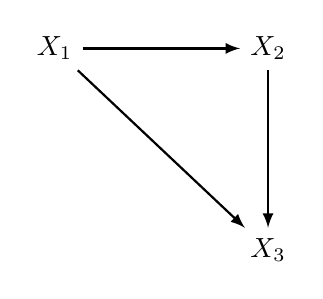
\begin{tikzpicture}[node distance=2cm, auto, >=latex, thick]
      \node (X1) {$X_1$};
      \node (X2) [right=of X1] {$X_2$};
      \node (X3) [below=of X2] {$X_3$};
      \draw[->] (X1) to (X2);
      \draw[->] (X2) to (X3);
      \draw[->] (X1) to (X3);
  \end{tikzpicture}
  \end{center}

  $X_3$ の構造方程式における $X_1$ の係数 $\beta_{31}$ を\textbf{直接効果}という.
  また，$X_1 \to X_2 \to X_3$ の有向道によって得られた $\beta_{32} \beta_{21}$ を\textbf{間接効果}という.

  より一般的に，構造方程式が以下で与えられるとする.
  \begin{align}
    \varepsilon_1, \varepsilon_2, \dots \varepsilon_n \overset{\text{i.i.d.}}{\sim} \mathcal{N}(0, 1) \\
    \begin{cases}
    X_1 = \varepsilon_1 \\
    X_2 = \beta_{21} X_1 + \varepsilon_2 \\
    \vdots \\
    X_m = \beta_{m, m-1} X_{m-1} + \varepsilon_m
    \end{cases}
  \end{align}
  このとき，
  \begin{equation}
    E[X_1 X_m] = \beta_{m, m-1} \cdot \beta_{m-1, m-2} \cdots \beta_{21}
  \end{equation}
  となり，これは $X_1$ から $X_m$ への間接効果である.
  総合効果こそ因果効果の大きさである.
\end{exm}

\begin{defn}[label={defn:TotalEffect}]{総合効果}
  構造方程式
  \begin{align}
    e &\sim \mathcal{N}(0, I_n) \\
    X &= BX + e
  \end{align}
  について，$n \times n$ 行列 $A$ を
  \begin{equation}
    A = (I - B)^{-1}
  \end{equation}
  とおいたときの $A$ の $(j, i)$ 成分 $a_{ji}$ を $X_i$ から $X_j$ への\textbf{総合効果}という.
\end{defn}

定義~\ref{defn:TotalEffect}の解釈は総合効果の本質を与える.
まず，$B$ は狭義下三角行列であるから冪零性により，
\begin{equation}
  (I - B)^{-1} = I + B + B^2 + \dots + B^{n-1}
\end{equation}
である.ここで$i<j$として$B^k$ の $(j, i)$ 成分 $b_{ji}^{(k)}$ に注目すると，
\begin{equation}
  b_{ji}^{(k)} = \sum_{l_{k-1}=1}^{n} \dots \sum_{l_1=1}^{n} \beta_{j, l_{k-1}} \beta_{l_{k-1}, l_{k-2}} \dots \beta_{l_1, i}
\end{equation}
となる.$B$ は狭義下三角行列であるため，
\begin{equation}
  b_{ji}^{(k)} = \sum_{i < l_1 < \dots < l_{k-1} < j} \beta_{j, l_{k-1}} \beta_{l_{k-1}, l_{k-2}} \dots \beta_{l_1, i}
\end{equation}
さて，各 $\beta_{j, l_{k-1}} \dots \beta_{l_1, i}$ が $0$ でない値を持つためには，任意の $\beta_{l_{m-1}, l_m}$ が $0$ でないことが条件となる.
これは，対応するDAGにおいて，
\begin{equation}
  X_i \to X_{l_1} \to \dots \to X_{l_{k-1}} \to X_j
\end{equation}
という長さ $k+1$ の有向道が存在することに等しい.
すなわち，$b_{ji}^{(k)}$ は $X_i$ から $X_j$ への長さ $k$ の有向道\footnote{第3章参照}によって得られる\textbf{間接効果}の和である.
したがって，
\begin{equation}
  (I - B)^{-1} = I + B + \dots + B^{n-1}
\end{equation}
の $(j, i)$ 成分は，長さ $1$ から $n$ の有向道によって得られる $X_i$ から $X_j$ への間接効果の和，つまり\textbf{総合効果}に等しい.

\begin{defn}[label={defn:ConfoundingEffect}]{交絡効果}
  構造方程式
  \begin{align}
    e &\sim \mathcal{N}(0, I_n) \\
    X &= BX + e
  \end{align}
  において，$A = (I - B)^{-1}$ としたときに，
  \begin{equation}
    C = AA^\top - (A + A^\top) + I
  \end{equation}
  の $(j, i)$ 成分 $c_{ji}$ を $X_i$ と $X_j$ の\textbf{交絡効果}という.
\end{defn}

定義~\ref{defn:ConfoundingEffect}\footnote{これは一般的な用語ではないことに注意されたい}を解釈しよう.まず，
\begin{equation}
  X = (I-B)^{-1}e = Ae
\end{equation}
より $X$ の分散共分散行列は，
\begin{align}
  E[XX^\top] &= E[(Ae)(Ae)^\top] \\
  &= A E[ee^\top] A^\top \\
  &= AA^\top
\end{align}
である.$i<j$として，$c_{ji}$ は $X_i$ と $X_j$ の共分散から，$X_i$ から $X_j$ への総合効果を引いたものである.
ここで，$A = (a_{ij})_{i,j=1}^n$ とおくと，
\begin{align}
  c_{ji} &= \sum_{k=1}^n a_{jk} a_{ik} - a_{ji} \\
  &= \sum_{k=1}^i a_{jk} a_{ik} - a_{ji} \\
  &= \sum_{k=1}^{i-1} a_{jk} a_{ik}
\end{align}
ここで，各 $k$ について，$a_{jk} a_{ik}$ は，$X_k$ から $X_i$ への総合効果と $X_k$ から $X_j$ への総合効果の積である.
これが $0$ でないときは，$X_k$ から $X_i$ への有向道が存在するかつ $X_k$ から $X_j$ への有向道が存在する場合(図\ref{fig:Confounding})である.
これは，$X_i$ と $X_j$ が共通の祖先を持つことを意味する\footnote{正確にはグラフ構造に対する忠実性の仮定が必要である}.
これは，例~\ref{exm:PseudoCorr}の擬似相関の概念を包含する概念である.

\begin{figure}[htbp]
  \centering
  \begin{tikzpicture}[
      node distance=2.5cm and 2.0cm,
      mynode/.style={circle, inner sep=2pt},
      arrow/.style={-{Stealth}, thick}
    ]
    \node[mynode] (Xk) {$X_k$};
    \node[mynode, below left=of Xk] (Xi) {$X_i$};
    \node[mynode, below right=of Xk] (Xj) {$X_j$};

    \node[inner sep=0pt, rotate=45] (dots1) at ($(Xk)!0.5!(Xi)$) {$\dots$};

    \draw[arrow, shorten >= 2pt] (Xk) -- (dots1);
    \draw[arrow, shorten <= 2pt] (dots1) -- (Xi);

    \node[inner sep=0pt, rotate=-45] (dots2) at ($(Xk)!0.5!(Xj)$) {$\dots$};
    
    \draw[arrow, shorten >= 2pt] (Xk) -- (dots2);
    \draw[arrow, shorten <= 2pt] (dots2) -- (Xj);
  \end{tikzpicture}
  \caption{交絡効果}
  \label{fig:Confounding}
\end{figure}


最後にパス係数の推定について少し触れよう.これまでは誤差項のパラメータは固定されていたが，推定論に関しては誤差項のパラメータも同時に推定する.
\begin{prop}{パス係数の推定}
  次の構造方程式を考える.
  \begin{equation}
      \varepsilon_1, \dots, \varepsilon_n \sim \mathcal{N}(\mu, \Psi)
  \end{equation}
  \begin{equation}
      \mu = (\mu_1, \dots, \mu_n), \quad \Psi = 
      \begin{pmatrix}
          \sigma_1^2 & & 0 \\
          & \sigma_2^2 & \\
          & & \ddots & \\
          0 & & & \sigma_n^2
      \end{pmatrix}
  \end{equation}
  \begin{equation}
      X = BX + e
  \end{equation}
  $B$ の非ゼロ成分を $\beta$ とおいて，$\theta = (\beta, \sigma_1^2, \dots, \sigma_n^2)$ とする.さらに，
  \begin{equation}
      \Sigma(\theta) = (I - B)^{-1} \Psi (I - B)^{-\top}
  \end{equation}
  とおいたときに，$\theta$ の最尤推定量 $\hat{\theta}$ は
  \begin{equation}
      f(\theta) = \text{tr}(\Sigma^{-1}(\theta) S) - \log(|\Sigma^{-1}(\theta) S|) - n
  \end{equation}
  を最小にする $\hat{\theta}$ として与えられる.ただし，$S$ は標本分散共分散行列である.
\end{prop}

\begin{proof}
  まず，
  \begin{equation}
      X = (I - B)^{-1} e
  \end{equation}
  より，$X \sim \mathcal{N}((I - B)^{-1} \mu, (I - B)^{-1} \Psi (I - B)^{-\top})$ である.
  ここで，標本 $x_1, \dots, x_N$ が与えられたとする.対数尤度関数は，
  \begin{align}
      -\log L(\theta) &= \frac{N}{2} \log (2\pi)^n |\Sigma(\theta)| + \frac{1}{2} \sum_{i=1}^N (x_i - \mu)^\top \Sigma^{-1}(\theta) (x_i - \mu) \\
      &= \frac{nN}{2} \log 2\pi - \log |\Sigma(\theta)|^{-1} + \frac{N}{2} \text{tr} \left( \Sigma^{-1}(\theta) \cdot \frac{1}{N} \sum_{i=1}^N (x_i - \mu)(x_i - \mu)^\top \right) \\
      &= \frac{nN}{2} \log 2\pi - \frac{N}{2} \log |\Sigma^{-1}(\theta)| + \frac{N}{2} \text{tr}(\Sigma^{-1}(\theta) S)
  \end{align}
  ゆえに，最尤推定量 $\hat{\theta}$ は，
  \begin{equation}
      -\log |\Sigma^{-1}(\theta)| + \text{tr}(\Sigma^{-1}(\theta) S)
  \end{equation}
  を最小化する $\theta$ として求められる.ここで，パラメータに関係ない項を加えて，
  \begin{align}
      f(\theta) &= \{ -\log |\Sigma^{-1}(\theta)| + \text{tr}(\Sigma^{-1}(\theta) S) \} - \log |S| - n \\
      &= \text{tr}(\Sigma^{-1}(\theta) S) - \log |\Sigma^{-1}(\theta) S| - n
  \end{align}
  を最小化する $\theta$ が最尤推定量である.
\end{proof}

\begin{exm}{}
  1.2で考えた構造方程式において最尤法でパラメータを推定する.以下に構造方程式の再掲と，最尤法によるパス係数の推定の結果を表\ref{tab:results_2}に記載する.
  \begin{align}
      &\varepsilon_X, \varepsilon_Y, \varepsilon_1, \dots, \varepsilon_6 \overset{\text{i.i.d.}}{\sim} N(0, 1) \\
      X  &= 0.6Z_1 + 0.6Z_5 + \varepsilon_X \\
      Y  &= X + 0.6Z_2 + 0.6Z_3 + 0.6Z_6 + \varepsilon_Y \\
      Z_1 &= 0.6Z_2 + \varepsilon_1 \\
      Z_2 &= \varepsilon_2 \\
      Z_3 &= 0.5X + \varepsilon_3 \\
      Z_4 &= 0.7X + 0.7Y + \varepsilon_4 \\
      Z_5 &= \varepsilon_5 \\
      Z_6 &= \varepsilon_6 
  \end{align}

  \begin{table}[H]
    \centering
    \caption{推定結果の要約}
    \label{tab:results_2}
    \begin{tabular}{lccc}
      \hline
      結果 & 関係 & 原因 & 推定値 \\ \hline
      Z1 & $\leftarrow$ & Z2 & 0.589887 \\
      X & $\leftarrow$ & Z1 & 0.601150 \\
      X & $\leftarrow$ & Z5 & 0.596700 \\
      Z3 & $\leftarrow$ & X & 0.486784 \\
      Y & $\leftarrow$ & X & 1.007328 \\
      Y & $\leftarrow$ & Z2 & 0.581893 \\
      Y & $\leftarrow$ & Z3 & 0.597675 \\
      Y & $\leftarrow$ & Z6 & 0.600582 \\
      Z4 & $\leftarrow$ & X & 0.707937 \\
      Z4 & $\leftarrow$ & Y & 0.698095 \\ \hline
    \end{tabular}
  \end{table}
\end{exm}

\newpage

\section{DAG}

\begin{defn}{有向グラフ}
  \begin{enumerate}
      \item 有限集合 $V$ と $V \times V$ の部分集合 $E$ の組 $(V, E)$ を（有限）グラフ， $V$ の要素を\textbf{頂点}， $E$ の要素を\textbf{辺}という.
      \item $(X_i, X_j) \in E$ かつ $(X_j, X_i) \notin E$ であるとき， $X_i$ から $X_j$ へ矢線を引く.一方で， $(X_i, X_j), (X_j, X_i) \in E$ のとき， $X_i$ と $X_j$ の間に向きのない辺を引く.
      \item すべての辺が向きのある辺のとき， $G$ を\textbf{有向グラフ}という.
  \end{enumerate}
\end{defn}

\begin{figure}[htbp]
  \begin{minipage}{0.45\textwidth}
    \centering
      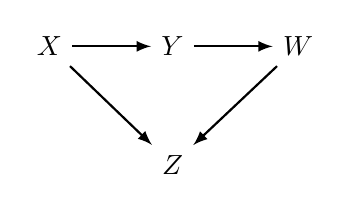
\begin{tikzpicture}[node distance=1cm, auto, >=latex, thick]
          \node (X) {$X$};
          \node (Y) [right=of X] {$Y$};
          \node (W) [right=of Y] {$W$};
          \node (Z) [below=of Y] {$Z$};
          \draw[->] (X) -- (Y);
          \draw[->] (Y) -- (W);
          \draw[->] (X) -- (Z);
          \draw[->] (W) -- (Z);
      \end{tikzpicture}
      \caption{有効グラフ}
  \end{minipage}
  \begin{minipage}{0.45\textwidth}
      \centering
      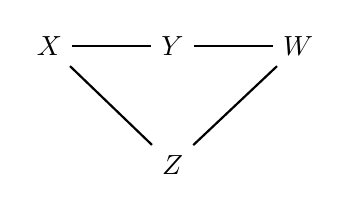
\begin{tikzpicture}[node distance=1cm, auto, thick]
          \node (X) {$X$};
          \node (Y) [right=of X] {$Y$};
          \node (W) [right=of Y] {$W$};
          \node (Z) [below=of Y] {$Z$};
          \draw[-] (X) -- (Y);
          \draw[-] (Y) -- (W);
          \draw[-] (X) -- (Z);
          \draw[-] (W) -- (Z);
      \end{tikzpicture}
      \caption{無向グラフ}
  \end{minipage}
\end{figure}

\begin{defn}{DAG}
$V = \{X_1, \dots, X_n\}$, $E \subset V \times V$, $G = (V, E)$ を有向グラフとする.
  \begin{enumerate}
      \item $X_i$ から $X_j$ への矢線が存在するとき， $X_i$ は $X_j$ の\textbf{親}であるといい， $X_j$ は $X_i$ の\textbf{子}であるという.また，
      \begin{equation}
          pa(X_j) = \{ X \in V \mid X \text{ は } X_j \text{ の親} \}
      \end{equation}
      と定義する.
      \item 頂点の列 $\{Y_i\}_{i=1}^m$ で，各 $i$ について， $Y_i$ から $Y_{i+1}$ または $Y_{i+1}$ から $Y_i$ への矢線が存在するとき， $\{Y_i\}_{i=1}^m$ を長さ $m$ の\textbf{道}という.とくに， $Y_i$ から $Y_{i+1}$ への矢線のみが存在する場合， $\{Y_i\}_{i=1}^m$ を\textbf{有向道}という.
      \item ある有向道 $\{Y_i\}_{i=1}^m$ が存在して， $Y_1 = Y_m$ となるとき，グラフ $G$ を\textbf{巡回グラフ}という.巡回グラフでない有向グラフを\textbf{非巡回有向グラフ}という.以下，非巡回有向グラフを \textbf{DAG} と表記する.
  \end{enumerate}
\end{defn}

\begin{figure}[H]
  \begin{minipage}{0.45\textwidth}
      \centering
      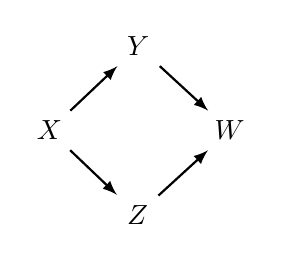
\begin{tikzpicture}[node distance=0.8cm, auto, >=latex, thick]
          \node (X) {$X$};
          \node (Y) [above right=of X] {$Y$};
          \node (Z) [below right=of X] {$Z$};
          \node (W) [below right=of Y] {$W$};
          \draw[->] (X) -- (Y);
          \draw[->] (Y) -- (W);
          \draw[->] (X) -- (Z);
          \draw[->] (Z) -- (W);
      \end{tikzpicture}
      \caption{巡回なし}
  \end{minipage}
  \begin{minipage}{0.45\textwidth}
      \centering
      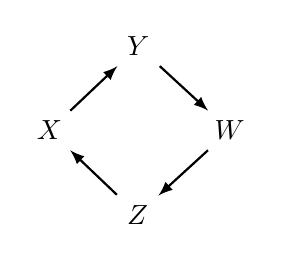
\begin{tikzpicture}[node distance=0.8cm, auto, >=latex, thick]
          \node (X) {$X$};
          \node (Y) [above right=of X] {$Y$};
          \node (Z) [below right=of X] {$Z$};
          \node (W) [below right=of Y] {$W$};
          \draw[->] (X) -- (Y);
          \draw[->] (Y) -- (W);
          \draw[->] (W) -- (Z);
          \draw[->] (Z) -- (X);
      \end{tikzpicture}
      \caption{巡回あり}
  \end{minipage}
\end{figure}

\newpage

\begin{defn}{子孫・先祖・合流点}
$V = \{X_1, \dots, X_n\}$, $E \subset V \times V$, $G = (V, E)$ は DAG であるとする.
  \begin{enumerate}
      \item 頂点 $X_i, X_j$ について，有向道 $\{Y_i\}_{i=1}^m, Y_1 = X_i, Y_m = X_j$ が存在するとき， $X_i$ は $X_j$ の\textbf{先祖}であるといい， $X_j$ は $X_i$ の\textbf{子孫}であるという.$X_i$ のすべての先祖を $an(X_i)$，すべての子孫を $de(X_i)$ で表す.
      \item すべての頂点から $X_i$ と $X_i$ の子孫を除いた頂点の部分集合を $nd(X_i)$ と書き， $nd(X_i)$ の要素を $X_i$ の\textbf{非子孫}という.
      \item 長さ $m$ の道 $\{Y_i\}_{i=1}^m$ について， $X_{j-1} \to X_j$ への矢線が存在し，かつ $X_{j+1} \to X_j$ への矢線が存在するとき， $X_j$ を\textbf{合流点（Collider）}という.とくに， $X_{j-1}$ と $X_{j+1}$ の間に辺が存在しないとき， $X_j$ を\textbf{V字合流点}という.
  \end{enumerate}
\end{defn}

\begin{exm}{子孫・非子孫・合流点}
  次の DAG を考える.
  \begin{center}
    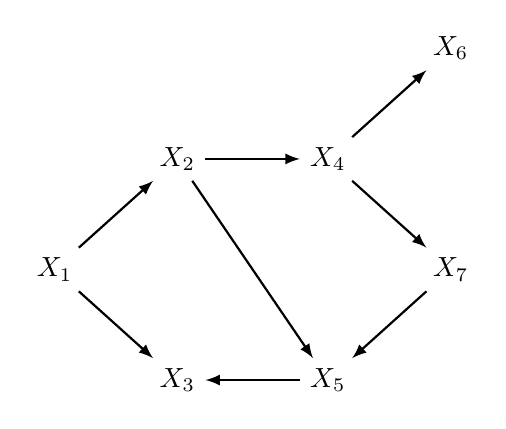
\begin{tikzpicture}[node distance=1.2cm, auto, >=latex, thick]
        \node (X1) {$X_1$};
        \node (X2) [above right=of X1] {$X_2$};
        \node (X3) [below right=of X1] {$X_3$};
        \node (X4) [right=of X2] {$X_4$};
        \node (X5) [right=of X3] {$X_5$};
        \node (X6) [above right=of X4] {$X_6$};
        \node (X7) [below right=of X4] {$X_7$};
        
        \draw[->] (X1) -- (X2);
        \draw[->] (X1) -- (X3);
        \draw[->] (X2) -- (X4);
        \draw[->] (X2) -- (X5);
        \draw[->] (X4) -- (X6);
        \draw[->] (X4) -- (X7);
        \draw[->] (X5) -- (X3);
        \draw[->] (X7) -- (X5);
    \end{tikzpicture}
  \end{center}

  \begin{enumerate}
      \item $X_1$ の子孫は？ $\Rightarrow \{X_2, X_3, X_4, X_5, X_6, X_7\}$
      \item $X_4$ の非子孫は？ $\Rightarrow \{X_1, X_2\}$
      \item 合流点は？ $\Rightarrow \{X_3, X_5\}$
  \end{enumerate}
\end{exm}

\begin{defn}{部分グラフ}
  $G = (V, E)$ をグラフとして，$V$ の部分集合 $U$ と
  \begin{equation}
    E_U = \{ (X_i, X_j) \in E \mid X_i, X_j \in U \}
  \end{equation}
  を定める.このとき，$G_U = (U, E_U)$ はグラフであり，$G_U$ を $U$ が生成する $G$ の\textbf{部分グラフ}であるという.
\end{defn}

\begin{prop}{}
  $G$ が DAG であれば，部分グラフ $G'$ も DAG である.\\
\end{prop}

\begin{proof}
  有向グラフであることと巡回がないことを証明すればよい.
  \begin{itemize}
      \item \textbf{有向グラフであること}：もし $(X_i, X_j) \in E', (X_j, X_i) \in E'$ であれば，$(X_i, X_j) \in E, (X_j, X_i) \in E$ となり，これは $G$ が有向グラフであることに矛盾する.
      \item \textbf{非巡回であること}：$G'$ が巡回グラフであるとすれば，有向道 $\{Y_i\}_{i=1}^m$ が存在する.ここで，各 $i$ について $Y_i \in V' \subset V$ かつ $(Y_i, Y_{i+1}) \in E' \subset E$ より，$\{Y_i\}_{i=1}^m$ は $G$ の有向道でもあるが，これは $G$ が非巡回であることに矛盾する.
  \end{itemize}
\end{proof}

\begin{defn}{祖先集合}
    DAG $G=(V,E)$の頂点の部分集合$U$が次の条件を満たすとき，$U$を祖先集合という.
    \[
       X \in U \Rightarrow pa(X) \subset U 
    \]  
\end{defn}

\begin{prop}[label={prop:AncestorSet}]{}
  $V=\{X_1, \dots, X_n\}$, $G=(V,E)$をDAGとする.任意の頂点$X_i \in V$について，$nd(X_i),nd(X_i) \cup \{X_i\}$は祖先集合である.
\end{prop}

\begin{proof}
  任意の頂点$X_j \in nd(X_i)$について，$X_j$から$X_i$への有向道が存在しない.
  したがって，$X_j$の任意の親から$X_i$への有向道は存在しないため，$pa(X_j) \subset nd(X_i)$.つまり，$nd(X_i)$は祖先集合である.
  さらに，非子孫の定義により$X_i$の親もすべて$nd(X_i)$に属する.ゆえに，$nd(X_i) \cup \{X_i\}$は祖先集合である.
\end{proof}

\begin{defn}{隣接行列}
  $G = (V, E)$ をグラフ，$V = \{X_1, \dots, X_n\}$ とする.$n \times n$ 行列 $A$ を
  \begin{equation}
    a_{ij} = 
    \begin{cases} 
      1 & (X_j, X_i) \in E \\
      0 & (X_j, X_i) \notin E 
    \end{cases}
  \end{equation}
  として，$A = (a_{ij})_{i,j=1}^n$ で定義する.この $A$ をグラフ $G$ の\textbf{隣接行列}という.
\end{defn}

とくに，$G$ が DAG である場合，隣接行列は冪零行列である.これを証明するために，いくつかの補題を準備しよう.

\begin{prop}[label={prop:TopoSort}]{トポロジカルソート}
  $G = (V, E)$ を DAG, $V = \{X_1, \dots, X_n\} \neq \emptyset$ とする.このとき，$X_1, \dots, X_n$ の順序を替えた $Y_1, \dots, Y_n$ であって，
  \begin{equation}
    (Y_i, Y_j) \in E \Rightarrow i < j
  \end{equation}
  となるようにできる.
\end{prop}

\begin{proof}
  まず，$pa(X_k) = \emptyset$ となる頂点 $X_k$ が存在することを証明する.\\
  任意の頂点 $X_i$ について $pa(X_i) \neq \emptyset$ と仮定する.
  $Z_1 \in V$ として，$pa(Z_1) \neq \emptyset$ より $(Z_2, Z_1) \in E$ となる $Z_2 \in V$ が存在.
  同様に $pa(Z_2) \neq \emptyset$ より $(Z_3, Z_2) \in E$ となる $Z_3 \in V$ が存在.
  これを繰り返すことで，有向道 $\{Z_i\}_{i=1}^{n+1}$ が存在する.一方で，$V$ の要素数は $n$ であったから，
  \begin{equation}
  Z_{i_1} = Z_{i_2}
  \end{equation}
  となる $i_1, i_2 \in \{1, \dots, n+1\}$ が存在する.これは $G$ が非巡回であることに矛盾する.

  さて，$V$ の要素数の帰納法によって補題を示す.このような規則でグラフの頂点の添字を付け替えることをトポロジカルソートという.
  \begin{itemize}
      \item $n=1$ のとき，$V$ は補題を満たす.
      \item $n=k$ のとき，$V$ は補題を満たすと仮定する.
      \item $n=k+1$ のとき，$G = (V, E)$ は DAG であるから，$pa(X_k) = \emptyset$ となる $X_k \in V$ が存在.
      このとき，$V' = V \setminus \{X_k\}$, $E' = \{ (X_i, X_j) \in E \mid X_i \neq X_k \text{ かつ } X_j \neq X_k \}$ とすれば，$G' = (V', E')$ は $G$ の部分グラフである.
      $G$ が DAG であったから $G'$ も DAG であって，要素数が $k$ である.
      ゆえに，$X_k = Y_1$ として，$V'$ をトポロジカルソートして $\{Y_i\}_{i=2}^{k+1}$ と並べ替えれば，$\{Y_i\}_{i=1}^{k+1}$ はトポロジカルソートされた頂点集合となる.
  \end{itemize}
\end{proof}

\begin{thm}{}
  グラフ $G$ が DAG である場合，隣接行列 $A$ は\textbf{狭義下三角行列に相似}である.
\end{thm}

\begin{proof}
  $V = \{X_1, \dots, X_n\}$ とする.$\{Y_i\}_{i=1}^n$ はトポロジカルソートされたものであるとする.
  $Y_1, \dots, Y_n$ は $X_1, \dots, X_n$ の並べ替えであるから，$Y_1 = X_{\pi(1)}, \dots, Y_n = X_{\pi(n)}$ となるような$n$ 次対称群 $S_n$ の元 $\sigma$ が存在する.
  ここで，$P = (e_{\sigma(1)}, \dots, e_{\sigma(n)})$ とおく.
  つまり，$P = (p_{ij})_{i,j=1}^n$ とおくと，
  \begin{equation}
    p_{ij} = 
    \begin{cases} 
      1 & (j = \sigma(i)) \\
      0 & (\text{otherwise})
    \end{cases}
  \end{equation}

  ここで，$PAP^\top$ の $(i, j)$ 成分を $a'_{ij}$ とおく.
  \begin{align}
    a'_{ij} &= \sum_{k=1}^n \sum_{l=1}^n p_{ik} a_{kl} p_{jl} \\
    &= \sum_{k=1}^n p_{ik} \left( \sum_{l=1}^n a_{kl} p_{jl} \right) \\
    &= \sum_{k=1}^n p_{ik} a_{k, \sigma(j)} = a_{\sigma(i), \sigma(j)}
  \end{align}

  $a_{\sigma(i), \sigma(j)}$ の定義より，
  \begin{align}
    a_{\sigma(i), \sigma(j)} &= 
    \begin{cases} 
      1 & (X_{\sigma(j)}, X_{\sigma(i)}) \in E \\
      0 & (\text{otherwise})
    \end{cases} \\
    &= 
    \begin{cases} 
      1 & (Y_j, Y_i) \in E \\
      0 & (\text{otherwise})
    \end{cases}
  \end{align}

  ゆえに，$PAP^\top$ は $\{Y_i\}_{i=1}^n$ のグラフの隣接行列 $A'$ に等しい.
  ここで，$\{Y_i\}_{i=1}^n$ はトポロジカルソートされているため，
  \begin{equation}
    (Y_j, Y_i) \in E \Rightarrow j < i
  \end{equation}
  ゆえに，$A'$ は狭義下三角行列である.したがって，隣接行列$A$は狭義下三角行列に相似である.
\end{proof}

\newpage

\section{ベイジアンネットワーク}

\begin{defn}[label={defn:BN}]{ベイジアンネットワーク}
  $G = (V, E)$ をDAG（有向非巡回グラフ）として，$V = \{X_1, \dots, X_n\}$ について，各 $X_i$ は確率変数である.
  $X_1, \dots, X_n$ の同時確率について，
  \begin{equation}
      P(X_1, \dots, X_n) = \prod_{i=1}^{n} P(X_i \mid pa(X_i))
  \end{equation}
  が成り立つとき，このモデルを\textbf{ベイジアンネットワーク}という.
\end{defn}

\begin{prop}[label={prop:ancestor}]{祖先集合におけるベイジアンネットワークの性質}
  確率変数 $X_1, \dots, X_n$ を頂点集合としたDAG $G = (V, E)$ を考える.
  このとき，任意の\textbf{祖先集合} $U$，つまり
  \begin{equation}
      X_i \in U \Rightarrow pa(X_i) \subset U
  \end{equation}
  となる $V$ の部分集合について，Uによって生成される部分グラフ$G_U$ はベイジアンネットワークである.
\end{prop}

\begin{proof}
  同時確率は以下のように分解できる.
  \begin{equation}
      P(X_1, \dots, X_n) = \prod_{X_i \in U} P(X_i \mid pa(X_i)) \cdot \prod_{X_j \notin U} P(X_j \mid pa(X_j))
  \end{equation}
  ここで，$P$ を $V \setminus U$ に含まれる確率変数で周辺化する.$U$ は祖先集合であるから，
  \begin{equation}
      X_i \in U \Rightarrow pa(X_i) \subset U
  \end{equation}
  が成り立つ.つまり，第一項の $\prod_{X_i \in U} P(X_i \mid pa(X_i))$ は $V \setminus U$ に含まれる確率変数を含まない.ゆえに，
  \begin{align*}
      P(U) &= \sum_{V \setminus U} P(X_1, \dots, X_n) \\
      &= \prod_{X_i \in U} P(X_i \mid pa(X_i)) \cdot \sum_{V \setminus U} \prod_{X_j \notin U} P(X_j \mid pa(X_j))
  \end{align*}
  ここで，$V \setminus U$ の要素をトポロジカルソートしたものを $\{Y_i\}_{i=1}^m$ とおくと，
  \begin{align*}
      \sum_{V \setminus U} \prod_{X_j \notin U} P(X_j \mid pa(X_j)) &= \sum_{Y_1, \dots, Y_m} \prod_{i=1}^{m} P(Y_i \mid pa(Y_i)) \\
      &= \sum_{Y_1, \dots, Y_{m-1}} \prod_{i=1}^{m-1} P(Y_i \mid pa(Y_i)) \cdot \sum_{Y_m} P(Y_m \mid pa(Y_m)) \\
      &= \sum_{Y_1, \dots, Y_{m-1}} \prod_{i=1}^{m-1} P(Y_i \mid pa(Y_i)) \cdot 1 \\
      &= \dots = 1
  \end{align*}
  したがって，
  \begin{equation}
      P(U) = \prod_{X_i \in U} P(X_i \mid pa(X_i))
  \end{equation}
  となり，$G_U$ はベイジアンネットワークの定義を満たす.
\end{proof}

\vspace{1em}
ベイジアンネットワークは次の\textbf{局所マルコフ性}で特徴づけられる.

\begin{defn}[label={defn:local_markov}]{局所マルコフ性}
  $V = \{X_1, \dots, X_n\}$ を確率変数の集合として，DAG $G = (V, E)$ を考える.
  任意の $X_i$ がその親を与えられたとき，親以外のすべての非子孫と独立になる，すなわち，
  \begin{equation}
      X_i \perp nd(X_i) \setminus pa(X_i) \mid pa(X_i)
  \end{equation}
  が成り立つとき，これを\textbf{局所マルコフ性}という.
\end{defn}

\begin{prop}{}
  ベイジアンネットワークは局所マルコフ性を持つ.逆に局所マルコフ性をもつ確率分布はベイジアンネットワークである.
\end{prop}

\begin{proof}
  まず，ベイジアンネットワークが局所マルコフ性を持つことを示す.
  命題\ref{prop:AncestorSet}により，$nd(X_i) \cup \{X_i\}$ は祖先集合であるから，命題\ref{prop:ancestor}より$G_{nd(X_i) \cup \{X_i\}}$ はベイジアンネットワークである.
  このとき，同時確率が次のように分解できる.
  \begin{align}
      P(nd(X_i) \cup \{X_i\}) &= \prod_{X_j \in nd(X_i) \cup \{X_i\}} P(X_j \mid pa(X_j)) \\
      P(nd(X_i)) &= \prod_{X_j \in nd(X_i)} P(X_j \mid pa(X_j))
  \end{align}
  よって，
  \begin{align}
      P(X_i \mid nd(X_i)) &= \frac{P(X_i,nd(X_i))}{P(nd(X_i))} \\
      &= \frac{\prod_{X_j \in nd(X_i) \cup \{X_i\}} P(X_j \mid pa(X_j))}{\prod_{X_j \in nd(X_i)} P(X_j \mid pa(X_j))} \\
      &= P(X_i \mid pa(X_i))
  \end{align}
  が成り立つ.ゆえに，
  \begin{align}
      P(X_i, nd(X_i) \setminus pa(X_i) \mid pa(X_i)) &= \frac{P(X_i, nd(X_i))}{P(pa(X_i))} \\
      &= \frac{P(X_i \mid nd(X_i)) \cdot P(nd(X_i))}{P(pa(X_i))} \\
      &= \frac{P(X_i \mid pa(X_i)) \cdot P(nd(X_i))}{P(pa(X_i))} \\
      &= P(X_i \mid pa(X_i)) \cdot P(nd(X_i) \mid pa(X_i)) \\
  \end{align}
  したがって，局所マルコフ性が証明される.
  次に，局所マルコフ性をもつ確率分布がベイジアンネットワークであることを示す.
  $V = \{X_1, \dots, X_n\}$ について，$V$ の要素をトポロジカルソートして $Y_1, \dots, Y_n$ と並べ替える.一般的に次の式が成り立つ.
  \begin{align}
      P(Y_1, \dots, Y_n) &= P(Y_1) \cdot P(Y_2 \mid Y_1) \cdots P(Y_n \mid Y_1, \dots, Y_{n-1}) \\
      &= \prod_{i=1}^{n} P(Y_i \mid Y_1, \dots, Y_{i-1})
  \end{align}
  ここで、$Y_1, \dots, Y_n$ はトポロジカルソートされているため$\{Y_1, \dots, Y_{i-1}\} \subset nd(Y_i)$ が成り立つ.
  ゆえに、局所マルコフ性より、
  \begin{equation}
      P(Y_i \mid Y_1, \dots Y_{i-1}) = P(Y_i \mid pa(Y_i))
  \end{equation}
  が成り立つ.したがって、
  \begin{align}
    P(Y_1, \dots, Y_n) &= \prod_{i=1}^{n} P(Y_i \mid Y_1, \dots, Y_{i-1}) \\
     &= \prod_{i=1}^{n} P(Y_i \mid pa(Y_i))
  \end{align}  
  したがって，$G$ はベイジアンネットワークである.
\end{proof}

局所マルコフ性は実質的に，
\begin{equation}
    P(X_i \mid nd(X_i)) = P(X_i \mid pa(X_i))
\end{equation}
を要請していることが分かる.これは，自分の非子孫，つまり「前の情報」による条件付き確率は，親で条件を付けるのと変わらないことを要求している.

\begin{defn}[label={defn:d-separation}]{有向分離 (d-separation)}
  $V = \{X_1, \dots, X_n\}$, $G = (V, E)$ として，ベイジアンネットワークを考える.
  頂点 $X_i, X_j$ を結ぶ道 $p$ を考える.$V$ の部分集合 $S$ が次の I, II の一方の条件を満たすとき，$S$ は道 $p$ を\textbf{ブロックする}という.

  \begin{enumerate}
      \item[I.] $p$ が $X_\alpha \to X_\beta \to X_\gamma$ または $X_\alpha \leftarrow X_\beta \to X_\gamma$ という経路を含み，かつ $S$ は $X_\beta$ を含む.
      \item[II.] $p$ が $X_\alpha \to X_\beta \leftarrow X_\gamma$ という経路（合流点）を含み，かつ $S$ は $X_\beta$ および任意の $X_\beta$ の子孫を含まない.
  \end{enumerate}

  $X_i, X_j$ を結ぶすべての道が $V$ の部分集合 $S$ によってブロックされているとき，$S$ は $X_i, X_j$ を\textbf{有向分離}するという.
\end{defn}

\begin{thm}[label={thm:global_markov}]{大域マルコフ性}
  ベイジアンネットワーク $V = \{X_1, \dots, X_n\}$, $G = (V, E)$ において，$X_i, X_j$ が $S \subset V$ によって有向分離されているとき，
  \begin{equation}
      X_i \perp X_j \mid S
  \end{equation}
  が成り立つ.
\end{thm}

\begin{exm}{}
  次のDAGを考える.

  \begin{center}
    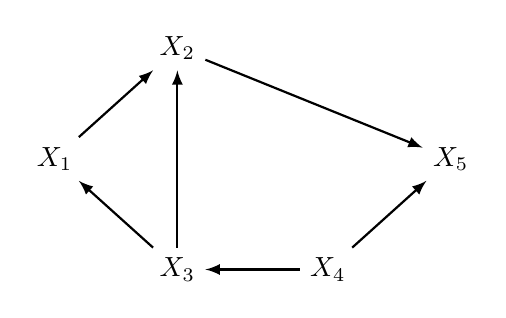
\begin{tikzpicture}[node distance=1.2cm, auto, >=latex, thick]
        \node (X1) {$X_1$};
        \node (X2) [above right=of X1] {$X_2$};
        \node (X3) [below right=of X1] {$X_3$};
        \node (X4) [right=of X3] {$X_4$};
        \node (X5) [above right=of X4] {$X_5$};
        
        \draw[->] (X1) -- (X2);
        \draw[->] (X3) -- (X1);
        \draw[->] (X3) -- (X2);
        \draw[->] (X4) -- (X3);
        \draw[->] (X4) -- (X5);
        \draw[->] (X2) -- (X5);
    \end{tikzpicture}
  \end{center}

  $X_1$ と $X_5$ を有向分離する $S$ を考える.$X_1$ と $X_5$ の道は：
  \begin{itemize}
      \item $p_1 : X_1 \to X_2 \to X_5$
      \item $p_2 : X_1 \leftarrow X_3 \leftarrow X_4 \to X_5$
      \item $p_3 : X_1 \leftarrow X_3 \to X_2 \to X_5$
      \item $p_4 : X_1 \to X_2 \leftarrow X_3 \leftarrow X_4 \to X_5$
  \end{itemize}

  このとき，$S$ は何か考えよう.
  まず，$p_1$ の構造は条件 I の連鎖構造であるから，$X_2 \in S$ でなければならない.
  一方，$p_4$ に着目すれば，$X_2$ は合流点である.ゆえに，$S$ が条件 II を満たすことはない.
  $p_2, p_3, p_4$ については条件 I を満たすように $S$ を定める.これらを考慮すれば，
  \begin{equation*}
      S = \{X_2, X_3\}
  \end{equation*}
  と求められる.ゆえに，定理~\ref{thm:global_markov}によれば，
  \begin{equation*}
      X_1 \perp X_5 \mid X_2, X_3
  \end{equation*}
  が成立する.
  ここで，
  \begin{align*}
      P(X_1, X_2, X_3, X_4, X_5) &= P(X_1 \mid X_3) P(X_2 \mid X_1, X_3) P(X_3 \mid X_4) P(X_4) P(X_5 \mid X_2, X_4)
  \end{align*}
  $X_4$ で周辺化すると，
  \begin{align*}
      P(X_1, X_2, X_3, X_5) &= P(X_1 \mid X_3) P(X_2 \mid X_1, X_3) \sum_{X_4} P(X_3 \mid X_4) P(X_4) P(X_5 \mid X_2, X_4)
  \end{align*}
  ここで，
  \begin{align*}
      \phi_1(X_1, X_2, X_3) &= P(X_1 \mid X_3) P(X_2 \mid X_1, X_3) \\
      \phi_2(X_5, X_2, X_3) &= \sum_{X_4} P(X_3 \mid X_4) P(X_4) P(X_5 \mid X_2, X_4)
  \end{align*}
  とおけば，
  \begin{equation}
      P(X_1, X_2, X_3, X_5) = \phi_1(X_1, X_2, X_3) \phi_2(X_5, X_2, X_3)
  \end{equation}
  となり，条件付き独立性が証明できる.
\end{exm}

定理~\ref{thm:global_markov}はベイジアンネットワークの理論における大定理であり，証明のためにいくつかの準備を要する.

\begin{defn}{無向グラフ}
  頂点集合 $V = \{X_1, \dots, X_n\}$ とグラフ $G = (V, E)$ において，
  \begin{equation}
      (X_i, X_j) \in E \Rightarrow (X_j, X_i) \in E
  \end{equation}
  が成り立つ，つまり，すべての辺に向きがない辺であるとき，$G$ を\textbf{無向グラフ}という.
\end{defn}

\begin{defn}{完全グラフ・クリーク}
  頂点集合 $V = \{X_1, \dots, X_n\}$，無向グラフ $G = (V, E)$ を考える.
  \begin{enumerate}
      \item 任意の頂点 $X_i, X_j$ が辺で結ばれているとき，グラフ $G$ は\textbf{完全グラフ}であるという.
      \item $V$ の部分集合 $C$ において，$C$ が生成する部分グラフ $G_C$ が完全グラフであるとき，$C$ を\textbf{クリーク}という.とくに，$C \subset U$ かつ $U$ がクリークである $U \subset V$ が存在しないとき，$C$ は\textbf{極大クリーク}であるという.
  \end{enumerate}
\end{defn}

\begin{exm}{}
  \begin{center}
    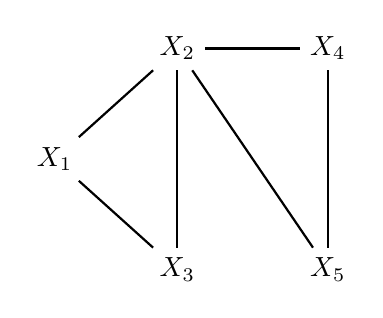
\begin{tikzpicture}[node distance=1.2cm, auto, >=latex, thick]
        \node (X1) {$X_1$};
        \node (X2) [above right=of X1] {$X_2$};
        \node (X3) [below right=of X1] {$X_3$};
        \node (X4) [right=of X2] {$X_4$};
        \node (X5) [right=of X3] {$X_5$};
        
        \draw[-] (X1) -- (X2);
        \draw[-] (X1) -- (X3);
        \draw[-] (X2) -- (X3);
        \draw[-] (X2) -- (X4);
        \draw[-] (X2) -- (X5);
        \draw[-] (X4) -- (X5);
    \end{tikzpicture}
  \end{center}

  $\{X_1, X_2, X_3\}, \{X_2, X_4, X_5\}$ は極大クリークである.
\end{exm}

\begin{defn}{道・連結・分離}
  頂点集合 $V = \{X_1, \dots, X_n\}$，無向グラフ $G = (V, E)$ を考える.
  \begin{enumerate}
      \item 頂点の列 $\{Y_i\}_{i=1}^m$ において，$(Y_{i-1}, Y_i) \in E$ となるとき，$\{Y_i\}_{i=1}^m$ を長さ $m$ の\textbf{道}という.
      \item 頂点 $X_i, X_j$ において，長さ $m$ の道 $\{Y_i\}_{i=1}^m$ が存在して，$Y_1 = X_i, Y_m = X_j$ となるとき，$X_i, X_j$ は\textbf{連結}しているという.すべての頂点の組が連結しているグラフを連結グラフ，連結していない頂点の組が存在するグラフを非連結グラフという.\\
      $G$ の部分集合 $U$ から生成される部分グラフ $G_U$ が連結グラフをなす極大な部分グラフ（任意の $U \subset U'$ について $G_{U'}$ が連結グラフでない）とき，$U$ を\textbf{連結成分}という.
      \item $S$ を $V$ の部分集合として，頂点 $X_i$ と $X_j$ を結ぶ任意の道 $p$ が，$S$ のある要素を含むとき，$S$ は $X_i$ と $X_j$ を\textbf{分離}するという.
  \end{enumerate}
  \end{defn}

  \begin{defn}{マルコフネットワーク}
  確率変数 $X_1, \dots, X_n$ を頂点とした $V = \{X_1, \dots, X_n\}$ と無向グラフ $G = (V, E)$ を考える.
  2つの辺のない頂点 $X_i, X_j$ が $V$ の部分集合 $S$ によって分離されているとき，
  \begin{equation}
      X_i \perp X_j \mid S
  \end{equation}
  が成立する.この性質を満足するモデルを\textbf{マルコフネットワーク}という.
\end{defn}

このマルコフネットワークの定義は大域マルコフ性と呼ばれる.マルコフネットワークは次の局所マルコフ性を持つ.

\begin{prop}{局所マルコフ性}
  マルコフネットワーク $V = \{X_1, \dots, X_n\}$, $G = (V, E)$ を考える.$X_i \in V$ に対して，
  \begin{align*}
      bd(X_i) &= \{X_j \in V \mid (X_i, X_j) \in E\} \\
      cl(X_i) &= \{X_i\} \cup bd(X_i)
  \end{align*}
  とおく.このとき，
  \begin{equation}
      X_i \perp V \setminus cl(X_i) \mid bd(X_i)
  \end{equation}
  が成り立つ.
\end{prop}

\begin{proof}
  定義より，$bd(X_i)$ は $X_i$ と $V \setminus cl(X_i)$ の任意の要素を分離する.
  ゆえに大域マルコフ性より，$X_j \in V \setminus cl(X_i)$ について，
  \begin{equation*}
      X_i \perp X_j \mid bd(X_i).
  \end{equation*}
  よって示された.
\end{proof}

\begin{thm}[label={thm:CliqueFactor}]{}
  確率変数 $X_1, \dots, X_n$ を頂点とした $V = \{X_1, \dots, X_n\}$ と無向グラフ $G = (V, E)$ を考える.
  $C_1, \dots, C_l$ をクリークとして，
  \begin{equation}
      V = \bigcup_{k=1}^l C_i
  \end{equation}
  とする.また，各 $C_i$ の要素を $X^{(k)}$ とおく.
  今，$X_1, \dots, X_n$ の同時確率が，
  \begin{equation}
      P(X_1, \dots, X_n) = \prod_{k=1}^l \phi_k(X^{(k)})
  \end{equation}
  と分解できるとする.このとき大域マルコフ性を満たす.
\end{thm}

\begin{proof}
  $X_i, X_j$ を辺がない任意の頂点，$S$ を分離集合とする.
  さて，集合 $V \setminus S$ において，$X_i$ を含む連結成分を $C(X_i)$ とおく.さらに
  \begin{equation*}
      D(X_i) = C(X_i) \cup S
  \end{equation*}
  とおく.一方，
  \begin{equation*}
      D(X_j) = V \setminus C(X_i)
  \end{equation*}
  とおく.ここで，$G$ の $S$ に含まれない任意のクリーク $C$ について考える.$C$ は $D(X_i), D(X_j)$ のいずれか一方の部分集合であることを示す.
  まず $C$ が $D(X_i), D(X_j)$ の少なくとも一方に含まれことを証明しよう.

  $C \not\subseteq D(X_i)$かつ$C \not\subseteq D(X_j)$ と仮定する.
  このとき、$X_c^{(1)} \notin D(X_i)$ かつ $X_c^{(2)} \notin D(X_j)$ となる元 $X_c^{(i)}, X_c^{(j)} \in C$ が存在する.
  $C$はクリークであるから、$X_c^{(1)}$と$X_c^{(2)}$の間に辺が存在する.
  ゆえに、$D^{c}(X_j)=C(X_i)$から$X_c^{(2)} \in C(X_i)$であり、連結成分の定義より$X_c^{(1)} \in C(X_i)$.これは、$X_i^{(1)} \in D(X_i)$ に矛盾する.
  次に、$C$ が $D(X_i), D(X_j)$ の両方に含まれないことを確認しよう.
  $D(X_i) \cap D(X_j) = S$と$C \notin S$より、$C$ は $D(X_i), D(X_j)$ の両方に含まることはない.
  以上により、$C$ は $D(X_i), D(X_j)$ のいずれか一方の部分集合であることが示された.
  
  ここで，
  \begin{equation*}
      \mathscr{C} = \{C_1, \dots, C_l\}
  \end{equation*}
  として，
  \begin{align*}
      \mathscr{C}_i &= \{ C \in \mathscr{C} \mid C \subseteq S \text{ または } C \subseteq D(X_i) \} \\
      \mathscr{C}_j &= \{ C \in \mathscr{C} \mid C \not\subseteq S \text{ かつ } C \subseteq D(X_j) \}
  \end{align*}
  とすれば，$\mathscr{C} = \mathscr{C}_i \cup \mathscr{C}_j, \mathscr{C}_i \cap \mathscr{C}_j = \phi$ となる.ここで，
  \begin{align*}
      P(X_1, \dots, X_n) &= \prod_{k=1}^{l} \phi_k(X^{(k)}) \\
      &= \prod_{C_k \in \mathscr{C}_i} \phi_k(X^{(k)}) \cdot \prod_{C_k \in \mathscr{C}_j} \phi_k(X^{(k)})
  \end{align*}
  さらに，
  \begin{align}
    C_k \in \mathscr{C}_i \Rightarrow C_k \cap (D(X_j) \setminus S) = \phi \\
    C_k \in \mathscr{C}_j \Rightarrow C_k \cap C(X_i) = \phi
  \end{align}     
  となるため，$\{X_i, X_j\} \cup S$ 以外で周辺化して，
  \begin{align*}
      \sum_{V \setminus \{X_i, X_j\} \cup S} P(X_1, \dots, X_n) &= \sum_{C(X_i) \setminus \{X_i\}} \sum_{D(X_j) \setminus S \cup \{X_j\}} \prod_{k=1}^l \phi_k(X^{(k)}) \\
      &= \sum_{C(X_i) \setminus \{X_i\}} \prod_{C_k \in \mathscr{C}_i} \phi_k(X^{(k)}) \cdot \sum_{D(X_j) \setminus S \cup \{X_j\}} \prod_{C_k \in \mathscr{C}_j} \phi_k(X^{(k)})
  \end{align*}
  \begin{align*}
      \psi_1(X_i, S) &= \sum_{C(X_i) \setminus \{X_i\}} \prod_{C_k \in \mathscr{C}_i} \phi_k(X^{(k)}) \\
      \psi_2(X_j, S) &= \sum_{D(X_j) \setminus S \cup \{X_j\}} \prod_{C_k \in \mathscr{C}_j} \phi_k(X^{(k)})
  \end{align*}
  とおけば，
  \begin{equation*}
      P(X_i, X_j, S) = \psi_1(X_i, S) \psi_2(X_j, S)
  \end{equation*}
  と分解できて，$X_i \perp X_j \mid S$ が言える.
\end{proof}

さて，定理~\ref{thm:CliqueFactor}によってマルコフネットワークにおいても同時確率の分解は，グラフの形が決定づけることが分かるが，ベイジアンネットワークの場合とはギャップがある.
次の無向グラフを考える.
\begin{equation*}
    X_1 - X_2 - X_3
\end{equation*}
これは，$X_2$ が $X_1, X_3$ を分離しているため，大域マルコフ性により，
\begin{equation*}
    X_1 \perp X_3 \mid X_2
\end{equation*}
同時確率で表せば，
\begin{equation*}
    P(X_1, X_2, X_3) = \phi_1(X_1, X_2) \phi_2(X_2, X_3)
\end{equation*}
と分解できることに等しい.一方で，この無向グラフを有向グラフとして考える場合は3通りの矢線の引き方が考えられる.

\begin{enumerate}
    \item $X_1 \to X_2 \to X_3$ \quad または \quad $X_1 \leftarrow X_2 \leftarrow X_3$
    \item $X_1 \leftarrow X_2 \to X_3$
    \item $X_1 \to X_2 \leftarrow X_3$
\end{enumerate}

これらをベイジアンネットワークと見て同時確率を分解すると，
\begin{enumerate}
    \item $P(X_1, X_2, X_3) = P(X_1) P(X_2 \mid X_1) P(X_3 \mid X_2) = P(X_1, X_2) P(X_3 \mid X_2)$
    \item $P(X_1, X_2, X_3) = P(X_1 \mid X_2) P(X_2) P(X_3 \mid X_2) = P(X_1, X_2) P(X_3 \mid X_2)$
    \item $P(X_1, X_2, X_3) = P(X_2 \mid X_1, X_3) P(X_1) P(X_3)$
\end{enumerate}

となる.まず興味深いのは，1, 2の同時分布はまったく同じである.つまり，データのみから1, 2のどちらの構造であるかを同定するのは非常に困難である.この難しさは後の因果探索の分野で触れる.

さて，無向グラフと有向グラフの同時確率が一致したのは1, 2の場合である.3の構造については，大域マルコフ性
\begin{equation*}
    X_1 \perp X_3 \mid X_2
\end{equation*}
が一般に成り立たない.むしろ3の場合は，
\begin{align*}
    P(X_1, X_2, X_3) &= P(X_2 \mid X_1, X_3) P(X_1) P(X_3) \\
    &= \frac{P(X_1, X_2, X_3)}{P(X_1, X_3)} P(X_1) P(X_3)
\end{align*}
より，$P(X_1, X_3) = P(X_1) P(X_3)$ となり，$X_1, X_3$ は独立であることが分かる.合流点においては，条件を付けることでむしろ独立性が崩れることがある.

合流点の構造をそのまま無向グラフにすると，条件付き独立性という誤った結論となる.このギャップを埋めるために，\textbf{モラル化}という操作を行う.

\begin{defn}{モラルグラフ}
  有向グラフ $G = (V, E)$ に対して，次のように構成される無向グラフを $G$ のモラルグラフといい，$G^m$ と表す.
  \begin{enumerate}
      \item $G^m$ の頂点集合は $V$
      \item $(X_i, X_j) \in E$ ならば，$G^m$ において $X_i$ と $X_j$ に辺を引く.
      \item 有向グラフ $G$ で $(X_i, X_k) \in E$ かつ $(X_j, X_k) \in E$ ならば，$G^m$ において $X_i$ と $X_j$ に辺を引く.
  \end{enumerate}
  とくに3の条件で引かれた辺を\textbf{モラルエッジ}という.
  また、有向グラフ$G$のモラルグラフ$G^m$を考えることを$G$を\textbf{モラル化}するという.
\end{defn}

\begin{figure}[h]
    \centering
    \begin{tikzpicture}[node distance=1.5cm, every node/.style={draw=none, inner sep=2pt}]
        % 有向グラフ G
        \node (x1) {$X_1$};
        \node (x2) [above right=of x1] {$X_2$};
        \node (x3) [below right=of x1] {$X_3$};
        \node (x4) [right=of x3] {$X_4$};
        \node (x5) [above right=of x4] {$X_5$};
        
        \path[->, thick] (x1) edge (x2);
        \path[->, thick] (x1) edge (x3);
        \path[->, thick] (x2) edge (x5);
        \path[->, thick] (x4) edge (x3);
        \path[->, thick] (x4) edge (x5);
        
        \node[draw=none, below=0.5cm of x3] {$G$: 有向グラフ};

        % 矢印
        \node[draw=none, right=6cm of x1] (arrow) {\huge $\Rightarrow$};

        % モラルグラフ Gm
        \begin{scope}[xshift=8.5cm]
            \node (m1) {$X_1$};
            \node (m2) [above right=of m1] {$X_2$};
            \node (m3) [below right=of m1] {$X_3$};
            \node (m4) [right=of m3] {$X_4$};
            \node (m5) [above right=of m4] {$X_5$};
            
            \path[thick] (m1) edge (m2);
            \path[thick] (m1) edge (m3);
            \path[thick] (m2) edge (m5);
            \path[thick] (m4) edge (m3);
            \path[thick] (m4) edge (m5);
            % モラル辺 (結婚)
            \path[thick] (m2) edge (m4); % X5の親同士を接続
            \path[thick] (m1) edge (m4); % X3の親同士を接続
            
            \node[draw=none, below=0.5cm of m3] {$G^m$: モラルグラフ};
        \end{scope}
    \end{tikzpicture}
\end{figure}

\begin{thm}[label={thm:MoralMarkov}]{大域マルコフ性とモラルグラフ}
  頂点集合 $V = \{X_1, \dots, X_n\}$ のベイジアンネットワーク $G = (V, E)$ が与えられているとする.
  このとき，$G$ をモラル化した $G^m$ とそのマルコフネットワークについて，$V$ の部分集合 $S$ が $X_i, X_j \in V$ を分離するとき，ベイジアンネットワーク $G$ において，
  \begin{equation}
      X_i \perp X_j \mid S
  \end{equation}
  が成り立つ.
\end{thm}

\begin{proof}
  ベイジアンネットワークの定義から，同時確率は
  \begin{equation}
      P(X_1, \dots, X_n) = \prod_{i=1}^n P(X_i \mid pa(X_i))
  \end{equation}
  と書ける.ここで，$\{X_i\} \cup pa(X_i)$ について，$X_i$ と $pa(X_i)$ の各要素には辺があり，モラルグラフの定義により，$pa(X_i)$ のどの2つの要素にも辺が存在するため，$\{X_i\} \cup pa(X_i)$ はクリークである.
  ゆえに，同時確率がクリーク毎の要素の関数の積で書けるため，定理~\ref{thm:CliqueFactor}より，$G^m$ は大域マルコフ性を持ち，マルコフネットワークとなる.
  ゆえに，$X_i, X_j \in V$ を $S \subseteq V$ が分離するとき，
  \begin{equation}
      X_i \perp X_j \mid S
  \end{equation}
  が成り立つ.
\end{proof}

定理 4.16 の本質は，同時確率 $P(X_1, \dots, X_n)$ が分解できることにある.これにより，より小さい $S$ によって，$X_i$ と $X_j$ の条件付き独立性が証明される.

\begin{cor}[label={cor:Markov}]{}
  頂点集合 $V = \{X_1, \dots, X_n\}$ のベイジアンネットワーク $G = (V, E)$ が与えられているとする.また，$X_i, X_j \in V$ と $S \subseteq V$ は互いに排反であるとする.
  このとき，$\{X_i\} \cup \{X_j\} \cup S$ を含む最小の祖先集合 $An(\{X_i\} \cup \{X_j\} \cup S)$ を考える.この祖先集合により生成される部分グラフのモラルグラフ $G^m_{An(\{X_i\} \cup \{X_j\} \cup S)}$ において，$S$ が $X_i$ と $X_j$ を分離するとき，
  \begin{equation}
      X_i \perp X_j \mid S
  \end{equation}
  が成り立つ.
\end{cor}

\begin{proof}
  命題~\ref{prop:ancestor}より，$G_{An(\{X_i\} \cup \{X_j\} \cup S)}$ はベイジアンネットワークであるから，定理~\ref{thm:MoralMarkov}により大域マルコフ性が証明される.
\end{proof}

この系~\ref{cor:Markov}を構成する $S$ こそ，定義~\ref{defn:d-separation}で述べた\textbf{有向分離}である.

\begin{thm}[label={thm:LauritzenForward}]{Lauritzen(1990)}
  頂点集合 $V = \{X_1, \dots, X_n\}$ のベイジアンネットワーク $G = (V, E)$ が与えられているとする.
  頂点 $X_i, X_j$ が $S \subset V$ によって有向分離されているとき，$S$ は無向グラフ $G^m_{An(\{X_i, X_j\} \cup S)}$ において $X_i$ と $X_j$ を分離する.
\end{thm}

\begin{proof}
  背理法を用いる．
  $S$ は無向グラフ $G^m_{An(\{X_i, X_j\} \cup S)}$ において $X_i$ と $X_j$ を分離していないと仮定する．
  つまり，ある道 $p = \{Y_k\}_{k=1}^m$ が $G^m_{An(\{X_i, X_j\} \cup S)}$ に存在して，どの $Y_k$ も $S$ の要素でない．
  $Y_k$ と $Y_{k+1}$ の辺を $e_k$（$k = 1, \dots, m-1$）とする．

  頂点の列 $\{Z_k\}_{k=1}^l$ を次のようにとる．
  \begin{enumerate}
    \item $Z_1 = Y_1$
    \item \begin{itemize}
      \item $e_1$ がモラルエッジでないとき，$Z_2 = Y_2$ とする．
      \item $e_1$ がモラルエッジのとき，$Y_1$ と $Y_2$ の $G$ における共通の子 $\gamma \in An(\{X_i\} \cup \{X_j\} \cup S)$ として $Z_2 = \gamma$，$Z_3 = Y_2$ とする．
    \end{itemize}
  \end{enumerate}
  $e_2, \dots, e_{m-1}$ においても同様に2のルールに従って頂点の列 $\{Z_k\}_{k=1}^l$ をとることができる．

  $p' = \{Z_k\}_{k=1}^l$ とすると，$Z_1 = Y_1 = X_i$，$Z_l = Y_m = X_j$ となり，$p'$ はグラフ $G$ における $X_i$ と $X_j$ の道である．

  ここで，道 $p'$ の非合流点はすべて $S$ の要素ではない．ゆえに，$p'$ は定義~\ref{defn:d-separation}の条件 I によってブロックされない．
  特に $p'$ に合流点が存在しない場合，$p'$ は $S$ によってブロックされない．これは $S$ が $X_i$ と $X_j$ を有向分離することに矛盾する．

  さて，すべての $Z_k$ は $An(\{X_i\} \cup \{X_j\} \cup S)$ の元であるから，$p'$ の任意の合流点 $\gamma$ について次のいずれかが成り立つ．
  \begin{itemize}
    \item[a)] $\gamma \in An(S)$
    \item[b)] $\gamma \notin An(S)$
  \end{itemize}

  \noindent\textbf{a) となる合流点が $p'$ に存在する場合：}
  $S$ は合流点の子孫を含むため，定義~\ref{defn:d-separation}の条件 II により $p'$ は $S$ によってブロックされない．これは $S$ が $X_i$ と $X_j$ を有向分離することに矛盾する．

  \noindent\textbf{$p'$ のすべての合流点が b) の場合：}
  道 $p'$ の合流点を $\gamma_1, \dots, \gamma_u$ とおく．このとき $\gamma_1, \dots, \gamma_u \in An(\{X_i, X_j\})$ である．
  $\gamma_1, \dots, \gamma_u$ の中で $An(X_i)$ に属するものの最大番号のものを $\gamma = Z_r$ とおく．

  $Z_r \in An(X_i)$ より，$Z_r$ から $X_i = Z_1$ への有向道 $\{W_k\}_{k=1}^t$（$W_1 = X_i$，$W_t = Z_r$）が存在する：
  \[
    W_1 \leftarrow W_2 \leftarrow \cdots \leftarrow W_t \leftarrow Z_{r+1} - \cdots - Z_l.
  \]
  $W_t = Z_r \notin An(S)$ より $W_1, \dots, W_t \notin S$ である．$Z_r$ の最大性により，$Z_{r+1}, \dots, Z_l$ に含まれる合流点はすべて $An(X_j)$ に属する．
  そのうち最小番号のものを $\gamma'' = Z_g$ とおく．$Z_g \in An(X_j)$ より，$Z_g$ から $X_j = Z_l$ への有向道 $\{W'_k\}_{k=1}^u$（$W'_1 = Z_g$，$W'_u = X_j$）が存在する：
  \[
    W_1 \leftarrow \cdots \leftarrow W_t \leftarrow Z_{r+1} - \cdots - Z_{g-1} \to W'_1 \to \cdots \to W'_u.
  \]
  $W'_1 = Z_g \notin An(S)$ より $W'_1, \dots, W'_u \notin S$．
  また，$Z_{r+1}, \dots, Z_{g-1}$ は $p'$ の非合流点であるから $S$ に属さない．
  道 $p'' = W_1, \dots, W_t, Z_{r+1}, \dots, Z_{g-1}, W'_1, \dots, W'_u$ においては，すべての頂点は $S$ に属さず，合流点も存在しない．
  ゆえに $S$ は道 $p''$ をブロックしない．

  以上のように，$S$ は $X_i$ と $X_j$ を有向分離することに矛盾する．
\end{proof}

定理~\ref{thm:LauritzenForward}は逆も成り立つことが知られている.

\begin{thm}[label={thm:LauritzenBackward}]{Lauritzen(1990)}
  頂点集合 $V = \{X_1, \dots, X_n\}$ のベイジアンネットワーク $G = (V, E)$ が与えられているとする.
  $S$ が無向グラフ $G^m_{An(\{X_i, X_j\} \cup S)}$ において $X_i$ と $X_j$ を分離するとき，頂点 $X_i, X_j$ が $S \subset V$ によって有向分離されている.
\end{thm}

\begin{proof}
  背理法を用いる.
  頂点集合 $S$ が $X_i, X_j$ を有向分離しないとき，
  つまり $X_i, X_j$ の道 $p = \{Y_k\}_{k=1}^m$ が存在して，$p$ は $S$ によってブロックされていない.
  $p$に合流点が存在しなければ，$p$ の任意の頂点は $S$ に含まれず、$S$は$X_i$と$X_j$を分離しない．

  このとき，$p$ の任意の合流点 $\gamma$ について，$\gamma$ または $\gamma$ の子孫が $S$ に含まれる.
  ゆえに，$\gamma \in An(S)$.
  さらに，$An(\gamma) \subset An(S)$ である.
  したがって，$p \subset An(S \cup \{X_i, X_j\})$.
  さて，この $p$ について，合流点以外は $S$ の元ではない.
  さらに，合流点については，モラル化することにより，合流点を含まない $G^m_{An(S \cup \{X_i, X_j\})}$ の道 $p'$ を構成できる.
\end{proof}

さて，以上の準備の下で定理~\ref{thm:global_markov}を証明しよう.\\
\textbf{定理~\ref{thm:global_markov}：大域マルコフ性}\\
ベイジアンネットワーク $V = \{X_1, \dots, X_n\}$, $G = (V, E)$ において，$X_i, X_j$ が $S \subset V$ によって有向分離されているとき，
\begin{equation}
    X_i \perp X_j \mid S
\end{equation}
が成り立つ.

\begin{proof}
  定理~\ref{thm:LauritzenForward}, \ref{thm:LauritzenBackward}により，$S$ は無向グラフ $G^m_{An(S \cup \{X_i, X_j\})}$ を（そのときに限り）分離する.
  ゆえに，系~\ref{cor:Markov}により，
  \begin{equation}
      X_i \perp X_j \mid S
  \end{equation}
  が成り立つ.
\end{proof}

\newpage

\section{介入・因果効果}

\begin{defn}{構造的因果モデル}
  $X_1, \dots, X_n$ を確率変数、$V = \{X_1, \dots, X_n\}$ を頂点集合とした DAG $G = (V, E)$ を考える。
  各 $X_i$ が可測関数 $f_i$ と誤差変数 $\varepsilon_i$ を用いて、
  $ X_i = f_i(pa(X_i), \varepsilon_i) $
  と記述されるとする。このとき、$G$ を\textbf{構造的因果モデル}という。
  ただし、誤差変数 $\varepsilon_i$ は外生的、つまり DAG $G' = (V \cup \{\varepsilon_1, \dots, \varepsilon_n\}, E \cup (\bigcup_{k=1}^n \{(\varepsilon_k, X_k)\})) $ とおいたときに、
  \begin{enumerate}
      \item 各 $i$ について、$pa(\varepsilon_i) = \emptyset$
      \item $i \neq j$ ならば、$\varepsilon_i \perp \varepsilon_j$
      \item $X_j \in nd(X_i)$ ならば、$\varepsilon_i \perp X_j$
  \end{enumerate}
  を仮定する。
\end{defn}

\begin{prop}{}
  構造的因果モデルはベイジアンネットワークである。
\end{prop}

\begin{proof}
  まず、$V' = \{X_1, \dots, X_n, \varepsilon_1, \dots, \varepsilon_n\}$ とした DAG $G'$ を考える。このとき、$\varepsilon_1, \dots, \varepsilon_n$ は親を持たず、各 $i$ について $X_i$ は $\varepsilon_i$ の子であることに注意する。

  ここで、任意の $X_i$ とその非子孫 $nd(X_i)$ の任意の要素 $U$ について、
  $ X_i \perp U \mid pa(X_i), \varepsilon_i $
  が成り立つ。ここで $pa(X_i)$ はグラフ $G$ における親であることに注意する。
  実際に、
  $ X_i = f_i(pa(X_i), \varepsilon_i) $
  であるため、$X_i \mid pa(X_i), \varepsilon_i$ は定数（決定論的に決まる）である。ゆえに、
  $ X_i \perp U \mid pa(X_i), \varepsilon_i $
  したがって、$G'$ は局所マルコフ性を持ち、ベイジアンネットワークである。$pa(\varepsilon_i) = \emptyset$ に注意して、
  $ P(X_1, \dots, X_n, \varepsilon_1, \dots, \varepsilon_n) = \prod_{i=1}^n P(X_i \mid pa(X_i), \varepsilon_i) P(\varepsilon_i) $
  さて、今 $X_1, \dots, X_n$ をトポロジカルソートして、$\varepsilon$ の番号と対応させたものとする。
  \begin{align}
    P(X_1, \dots, X_n) &= \sum_{\varepsilon_1, \dots, \varepsilon_n} P(X_1, \dots, X_n, \varepsilon_1, \dots, \varepsilon_n) \\
    &= \sum_{\varepsilon_1, \dots, \varepsilon_n} \prod_{i=1}^n P(X_i \mid pa(X_i), \varepsilon_i) P(\varepsilon_i) \\
    &= \sum_{\varepsilon_1, \dots, \varepsilon_n} \prod_{i=1}^n P(X_i, \varepsilon_i \mid pa(X_i)) \\
    &= \sum_{\varepsilon_1, \dots, \varepsilon_{n-1}} \prod_{i=1}^{n-1} P(X_i, \varepsilon_i \mid pa(X_i)) \cdot \sum_{\varepsilon_n} P(X_n, \varepsilon_n \mid pa(X_n)) \\
    &= \dots \\
    &= \prod_{i=1}^n P(X_i \mid pa(X_i))
  \end{align}
  となり、$G$ はベイジアンネットワークの定義を満たす。
\end{proof}

\begin{defn}{介入}
  DAG $G=(V,E)$, $V=\{X_1, \dots, X_n\}$ で、$G$ は構造的因果モデル、すなわち、各 $j \in \{1, \dots, n\}$ について、$X_j$ の親 $pa(X_j)$ と誤差変数 $\varepsilon_j$, 関数 $f_j$ を用いて、
  \begin{equation}
    X_j = f_j(pa(X_j), \varepsilon_j)
  \end{equation}
  と記述されるとする。このとき、ある $i$ について、定数 $x_i$ を用いて、
  \begin{equation}
    X_i = x_i
  \end{equation}
  と書き換える。この新しいメカニズムによって記述される構造的因果モデル $G_{\overline{X_i}}$ に基づく確率を
  \[
    P(X_1, \dots, X_n \mid do(X_i = x_i))
  \]
  で表し、この操作を $X_i$ についての介入という。
\end{defn}

さて、この介入後の分布 $P(X_1, \dots, X_n \mid do(X_i = x_i))$ はベイジアンネットワークであることが保証されているから、同時確率は次のように分解できる。
\begin{align*}
  P(X_1, \dots, X_n \mid do(X_i = x_i)) &= \prod_{j=1}^n P(X_j \mid pa(X_j)) \\
  &= \prod_{j=1, j \neq i}^n P(X_j \mid pa(X_j)) \cdot P(X_i \mid pa(X_i))
\end{align*}
ここで、
$X_i = x_i$より、$X_i \perp pa(X_i)$ であって、
\begin{align}
  P(X_i \mid pa(X_i)) = P(X_i) = \delta(x_i) = 
  \begin{cases} 
    1 & (X_i = x_i) \\ 
    0 & (X_i \neq x_i) 
  \end{cases}
\end{align}
となるから、
\begin{align}
  P(X_1, \dots, X_n \mid do(X_i = x_i)) &= \prod_{j=1, j \neq i}^n P(X_j \mid pa(X_j)) \cdot \delta(x_i) \\
  &= 
  \begin{cases} 
    \prod_{j=1, j \neq i}^n P(X_j \mid pa(X_j)) & (X_i = x_i) \\ 
    0 & (X_i \neq x_i) 
  \end{cases}
\end{align}
と書ける。
介入前と介入後の構造的因果モデルにおける確率変数は異なる確率変数であることに注意する。
なお、$X_i$ の非子孫については、生成過程に影響を与えず、同一の確率変数と考えてよい。

では $G$ と $G_{\overline{X_i}}$ をグラフとして比較してみよう。
$G_{\overline{X_i}}$ は、$X_i$ と $pa(X_i)$ が独立、つまり、グラフ上において、$pa(X_i)$ から $X_i$ への矢線をすべて排除した形になる。

\begin{exm}{}
  次のDAGから生成される構造的因果モデルを考える。
  \begin{figure}[H]
    \centering
    \begin{tikzpicture}[node distance=1.5cm, every node/.style={draw=none, inner sep=2pt}]
        % 有向グラフ G
        \node (x1) {$X_1$};
        \node (x2) [above right=of x1] {$X_2$};
        \node (x3) [below right=of x1] {$X_3$};
        \node (x4) [below right=of x2] {$X_4$};
        
        \path[->, thick] (x2) edge (x1);
        \path[->, thick] (x2) edge (x4);
        \path[->, thick] (x1) edge (x4);
        \path[->, thick] (x1) edge (x3);
        \path[->, thick] (x3) edge (x4);
        
        \node[draw=none, below=0.5cm of x3] {$G$: 介入前のグラフ};

        % 矢印
        \node[draw=none, right=4cm of x1] (arrow) {\huge $\Rightarrow$};

        % モラルグラフ Gm
        \begin{scope}[xshift=6cm]
            \node (m1) {$X_1=x_1$};
            \node (m2) [above right=of m1] {$X_2$};
            \node (m3) [below right=of m1] {$X_3$};
            \node (m4) [below right=of m2] {$X_4$};
            
            \path[->,thick] (m1) edge (m3);
            \path[->,thick] (m1) edge (m4);
            \path[->,thick] (m2) edge (m4);
            \path[->,thick] (m3) edge (m4);
            
            \node[draw=none, below=0.5cm of m3] {$G_{\overline{X_1}}$: 介入後のグラフ};
        \end{scope}
    \end{tikzpicture}
\end{figure}
  介入 $do(X_1 = x_1)$ を行った $G_{\overline{X_1}}$ を考える.
  $G$ と $G_{\overline{X_1}}$ を比較すれば、$X_2 \to X_1$ の矢線が消えていることが分かる。つまり、$G_{\overline{X_1}}$ の分布においては、$X_1$ と $X_4$ に共通の祖先は存在せず、交絡は存在しないことが分かる。
\end{exm}

次に因果効果の定義を与えよう。
\begin{defn}{平均因果効果}
  DAG $G=(V,E)$ は構造的因果モデルとする。このとき、$Y, X \in V$ について、$X=x_1$ から $X=x_2$ に介入したときの $Y$ への平均因果効果を
  \begin{equation}
    E[Y \mid do(X=x_1)] - E[Y \mid do(X=x_2)]
  \end{equation}
  で定義する。ただし、
  \begin{equation}
    E[Y \mid do(X=x)] = \sum_Y Y P(Y \mid do(X=x))
  \end{equation}
  である。とくに、$X$ が二値 $\{0, 1\}$ をとる確率変数であるとき、
  \begin{equation}
    E[Y \mid do(X=1)] - E[Y \mid do(X=0)]
  \end{equation}
  を平均処置効果（ATE）という。
\end{defn}

\begin{defn}{同時介入}
  DAG $G=(V,E)$, $V=\{X_1, \dots, X_n\}$ で、$G$ は構造的因果モデル、すなわち、各 $j \in \{1, \dots, n\}$ について、$X_j$ の親 $pa(X_j)$ と誤差変数 $\varepsilon_j$, 関数 $f_j$ を用いて、
  \begin{equation}
    X_j = f_j(pa(X_j), \varepsilon_j)
  \end{equation}
  と記述されるとする。このとき、ある $i_1, \dots, i_k$ について、定数 $x_{i_1}, \dots, x_{i_k}$ を用いて、
  \begin{equation}
    X_{i_1} = x_{i_1}, \dots, X_{i_k} = x_{i_k}
  \end{equation}
  と書き換える。この新しいメカニズムによって記述される構造的因果モデルに基づく確率を
  \begin{equation}
    P(X_1, \dots, X_n \mid do(X_{i_1}=x_{i_1}), \dots, do(X_{i_k}=x_{i_k}))
  \end{equation}
  で表し、この操作を $X_{i_1}, \dots, X_{i_k}$ についての同時介入という。このとき、同時確率は、
  \begin{align}
    &P(X_1, \dots, X_n \mid do(X_{i_1}=x_{i_1}), \dots, do(X_{i_k}=x_{i_k})) \notag \\
    &= \begin{cases} 
      \prod_{j \notin \{i_1, \dots, i_k\}} P(X_j \mid pa(X_j)) & (X_{i_1}=x_{i_1}, \dots, X_{i_k}=x_{i_k}) \\ 
      0 & (\text{otherwise}) 
    \end{cases}
  \end{align}
  となる。
\end{defn}

\begin{defn}{変数としての介入}
  DAG $G=(V,E)$, $V=\{X_1, \dots, X_n\}$ で、$G$ は構造的因果モデル、すなわち、各 $j \in \{1, \dots, n\}$ について、$X_j$ の親 $pa(X_j)$ と誤差変数 $\varepsilon_j$, 関数 $f_j$ を用いて、
  \begin{equation}
    X_j = f_j(pa(X_j), \varepsilon_j)
  \end{equation}
  と記述されるとする。このとき、$\{idle, x_i\}$ の値をとる外生変数 $F_i$ を用いて、
  \begin{align}
    X_i &= \hat{f}_i(pa(X_i), \varepsilon_i, F_i) \notag \\
    &= \begin{cases} 
      x_i & (F_i = x_i) \\ 
      f_i(pa(X_i), \varepsilon_i) & (F_i = idle) 
    \end{cases}
  \end{align}
  と書き換える。$V' = \{X_1, \dots, X_n, F_i\}$, $E' = E \cup \{(F_i, X_i)\}$ としたときに、$G' = (V', E')$ は構造的因果モデルであり、この $G'$ を\textbf{拡張ネットワーク}という。
\end{defn}

なお、同時介入についても拡張ネットワークは同様に定義できる。

$G'$ は定義から、$F_i = idle$ であれば $G$ に、$F_i = x_i$ であれば $G_{\overline{X_i}}$ に等しくなる。つまり、
\begin{equation}
  P(X_1, \dots, X_n \mid do(X_i = x_i)) = P(X_1, \dots, X_n \mid F_i = x_i)
\end{equation}
となる。
我々が観測できるのは $G$ に基づく分布 $P(X_1, \dots, X_n)$ であるが、介入効果を知りたいときは、$G_{\overline{X_i}}$ に基づく分布 $P(X_1, \dots, X_n \mid do(X_i = x_i))$ を観察によって得られる分布 $P(X_1, \dots, X_n)$ やその周辺分布で書き下す必要がある。
次のバックドア基準は、その十分条件を与える。

\begin{prop}{バックドア基準}
  確率変数 $X_1, \dots, X_n$、頂点集合 $V = \{X_1, \dots, X_n\}$、DAG $G = (V, E)$ で $G$ は構造的因果モデルとする。
  $Y, X \in V$ について、$X$ と $Y$ の道であり、$X$ への矢線がある道を\textbf{バックドアパス}という。
  $V$ の部分集合 $Z$ がすべてのバックドアパスをブロックするとき、$Z$ はバックドア基準を満たすという。このとき、
  \begin{equation}
    P(Y \mid do(X=x)) = \sum_z P(Y \mid X=x, Z) P(Z)
  \end{equation}
  が成り立つ。
\end{prop}

\begin{proof}
  拡張ネットワーク $G' = (V', E'), V' = V \cup \{F_x\}, E' = E \cup \{(F_x, X)\}$ を考える。
  さて、$F_x$ から $Y$ へのパスは $X$ を通るパスのみである。$X, Y$ のバックドアパスを含む場合、$Z$ によって、そうでない場合は $X$ で条件をつけることで、$F_x$ と $Y$ を有向分離できるため、定理~\ref{thm:global_markov}より、
  \begin{equation}
    F_x \perp Y \mid X, Z
  \end{equation}
  が成り立つ。ため、
  \begin{equation}
    P(Y \mid F_x=x, X=x, Z) = P(Y \mid F_x=idle, X=x, Z)
  \end{equation}
  となり、
  \begin{equation}
    P(Y \mid do(X=x), Z) = P(Y \mid X=x, Z)
  \end{equation}
  また、$Z$ は $X$ の子孫でないため、$F_x$ の子孫ではない。$F_x$ の親は空集合であるから局所マルコフ性により、
  \begin{equation}
    Z \perp F_x
  \end{equation}
  となるため、
  \begin{equation}
    P(Z \mid do(X=x)) = P(Z \mid F_x=x) = P(Z)
  \end{equation}
  以上により、
  \begin{align}
    P(Y \mid do(X=x)) &= P(Y \mid F_x=x) \notag \\
    &= \sum_z P(Y \mid F_x=x, Z) P(Z \mid F_x=x) \notag \\
    &= \sum_z P(Y \mid X=x, Z) P(Z)
  \end{align}
\end{proof}

\begin{exm}{IPW推定}
  バックドア基準は $Y \mid do(X=x)$ という介入の分布を、$P(Y \mid X=x, Z)P(Z)$ という観察データを用いた分布で書き下すことを可能にする。ここで、$Y \mid do(X=x)$ の平均を求めてみよう。
  \begin{align}
    E[Y \mid do(X=x)] &= \sum_y y P(Y \mid do(X=x)) \notag \\
    &= \sum_y y \sum_z P(Y \mid X=x, Z) P(Z) \notag \\
    &= \sum_y \sum_z y \cdot \frac{P(Y, X=x, Z)}{P(X=x, Z)} \cdot P(Z) \notag \\
    &= \sum_x \sum_y \sum_z y \cdot \frac{I(X=x) \cdot P(Y, X, Z)}{P(X=x \mid Z)} \notag \\
    &= E\left[ \frac{Y I(X=x)}{P(X=x \mid Z)} \right]
  \end{align}
  分母の $P(X=x \mid Z)$ は傾向スコアと呼ばれ、$e(Z)$ で表す。今、標本 $(x_1, y_1, z_1), \dots, (x_n, y_n, z_n)$ について、推定値
  \begin{equation}
    \frac{1}{n} \sum_{i=1}^n \frac{y_i I(x_i=x)}{e(z_i)}
  \end{equation}
  は $E[Y \mid do(X=x)]$ の一致かつ不偏な推定値を与える。これは Rubin 流でよく知られた \textbf{IPW推定法}である。
\end{exm}

\newpage
\begin{thebibliography}{9}

\bibitem{Pearl2009}
J. Pearl著，黒木学訳，『統計的因果推論 ―モデル・推論・推測―』，共立出版，2009.

\bibitem{Miyakawa2004}
宮川雅巳著，『統計的因果推論 ―回帰分析の新しい枠組み―』，朝倉書店，2004.

\bibitem{Miyakawa1998}
宮川雅巳著，『グラフィカルモデル』，朝倉書店，1997.

\bibitem{Lauritzen1990Networks}
S. L. Lauritzen, A. P. Dawid, B. N. Larsen, and H. G. Leimer, ``Independence properties of directed Markov fields,'' \textit{Networks}, Vol.~20, No.~5, pp.~491--505, 1990.

\end{thebibliography}
\end{document}